% Compile from the repository root: latexmk -pdf main.tex
% Overleaf: set main.tex as the main document; compiler = pdfLaTeX.
\documentclass[a4paper,12pt,oneside,openany]{report}

% Thesis identity and submission layout settings.
\newcommand{\thesistitle}{JHQ-GPU: Representation-Aware GPU ANN Search and Workload-Level Refinement Calibration}
\newcommand{\thesisshorttitle}{JHQ-GPU}
\newcommand{\thesissubtitle}{Representation-Aware GPU ANN Search\\and Workload-Level Refinement Calibration}
\newcommand{\thesisauthor}{Rui Luo}
\newcommand{\thesissupervisor}{Dr Mengxuan Zhang}
\newcommand{\thesiscourse}{COMP8800 --- Advanced Computing Research Project}
\newcommand{\thesisschool}{School of Computing}
\newcommand{\thesisuniversity}{The Australian National University}
\newcommand{\thesisdate}{October 2026}
% Optional: enter your student number if required by Canvas; blank hides it.
\newcommand{\thesisstudentnumber}{}

% The final build rejects unresolved writing or figure placeholders.
\newif\ifdraftthesis
\draftthesisfalse

% School of Computing long-thesis structure, with documented electronic-copy adaptations.
\usepackage[T1]{fontenc}
\usepackage[utf8]{inputenc}
\usepackage[english]{babel}
\usepackage{lmodern}
\usepackage{microtype}
\usepackage{geometry}
\usepackage{setspace}
\usepackage{xcolor}
\definecolor{ThesisNavy}{HTML}{18344A}
\definecolor{DraftColour}{HTML}{8A4515}
\usepackage{graphicx}
\graphicspath{{figures/}}
\usepackage{amsmath,amssymb,amsthm}
\usepackage{booktabs,array,tabularx,longtable}
\usepackage{caption,subcaption}
\captionsetup{font=small,labelfont=bf}
\captionsetup[table]{position=top}
\usepackage{enumitem}
\setlist{itemsep=0.2em,topsep=0.35em}
\usepackage{listings}
\lstset{basicstyle=\small\ttfamily,breaklines=true,
  columns=fullflexible,keepspaces=true,showstringspaces=false,
  frame=single,rulecolor=\color{black!20},tabsize=2}
\usepackage{tikz}
\usetikzlibrary{arrows.meta,positioning,decorations.pathreplacing}
\usepackage[numbers,sort&compress]{natbib}
\renewcommand{\bibfont}{\small\raggedright}
\usepackage[automark,headsepline]{scrlayer-scrpage}
% KOMA-Script long-thesis adaptation; see FORMAT_NOTES.txt for the ANU source.
% Independently configured with public KOMA interfaces; no third-party template source is redistributed.
% Keep the existing font size and margins. Normal leading follows the school template.
\geometry{a4paper,left=27mm,right=27mm,top=28mm,bottom=28mm,
  headheight=18pt,headsep=7mm,footskip=12mm}
\setstretch{1.0}
% Classic thesis paragraphs: indent instead of a half-line blank between them.
\setparsizes{1.2em}{0pt plus .5pt}{0pt plus 1fil}
% Preserve the existing, scoped roman math subscripts without rewriting equations.
\DeclareOldFontCommand{\rm}{\normalfont\rmfamily}{\mathrm}

% Mathematical statements and proofs share the body-text margins. Their
% headings occupy a separate line; upright statements distinguish prose from
% the mathematical symbols without switching whole paragraphs to italics.
\newtheoremstyle{thesis}
  {6pt plus 1pt minus 1pt}{4pt plus 1pt minus 1pt}
  {\normalfont\setlength{\parindent}{0pt}}{0pt}
  {\normalfont\bfseries}{.}{\newline}{}
\theoremstyle{thesis}
\makeatletter
\renewenvironment{proof}[1][\proofname]{%
  \par\pushQED{\qed}\normalfont
  \setlength{\parindent}{0pt}\setlength{\listparindent}{0pt}%
  \setlength{\parskip}{2pt plus .5pt}%
  \topsep4\p@\@plus\p@\@minus\p@\relax
  \trivlist
  \item[\hskip\labelsep\normalfont\bfseries #1\@addpunct{.}]%
  \leavevmode\par\nobreak\noindent\ignorespaces
}{%
  \popQED\endtrivlist\@endpefalse
}
\makeatother
% Each current statement/proof pair fits comfortably on one page. Keep the
% short pairs together so floats and page breaks cannot separate their parts.
\newenvironment{resultblock}{%
  \par\addvspace{6pt}\noindent\begin{minipage}[t]{\linewidth}%
}{%
  \end{minipage}\par\addvspace{6pt}%
}

\KOMAoptions{chapterprefix=false,headings=normal,numbers=noendperiod}
\setkomafont{disposition}{\normalfont\bfseries}
\setkomafont{chapter}{\normalfont\Large\bfseries}
\setkomafont{chapterprefix}{\normalfont\large\bfseries}
\RedeclareSectionCommand[beforeskip=1.5ex plus .3ex minus .2ex,
  afterskip=.8ex plus .2ex]{chapter}
\RedeclareSectionCommand[beforeskip=1.8ex plus .4ex minus .2ex,
  afterskip=.7ex plus .2ex]{section}
\RedeclareSectionCommand[beforeskip=1.4ex plus .3ex minus .2ex,
  afterskip=.6ex plus .2ex]{subsection}
\RedeclareSectionCommand[runin=true,beforeskip=.9ex plus .3ex minus .1ex,
  afterskip=.75em]{paragraph}

\clearpairofpagestyles
\automark[chapter]{chapter}
\ihead{\headmark}
\cfoot[\pagemark]{\pagemark}
\setkomafont{pageheadfoot}{\normalfont\footnotesize\color{black!65}}
\setkomafont{pagenumber}{\normalfont\small\color{black}}
\pagestyle{scrheadings}

\captionsetup{font={small,stretch=1.0},labelfont=bf,labelsep=period,
  justification=raggedright,singlelinecheck=false,skip=5pt}
\captionsetup[table]{position=top,skip=4pt}
\setlength{\textfloatsep}{12pt plus 2pt minus 2pt}
\setlength{\floatsep}{10pt plus 2pt minus 2pt}
\setlength{\intextsep}{10pt plus 2pt minus 2pt}
% Keep neighbouring floats together on float-only pages.
\makeatletter
\setlength{\@fptop}{0pt}
\setlength{\@fpsep}{12pt plus 2pt minus 2pt}
\setlength{\@fpbot}{0pt plus 1fil}
\makeatother
\setlength{\abovecaptionskip}{5pt}
\setlength{\belowcaptionskip}{0pt}
\setlist{itemsep=.15em,topsep=.35em,parsep=0pt}
\setlength{\bibsep}{.3em}
\setlength{\abovedisplayskip}{8pt plus 2pt minus 2pt}
\setlength{\belowdisplayskip}{8pt plus 2pt minus 2pt}
\setlength{\abovedisplayshortskip}{4pt plus 1pt}
\setlength{\belowdisplayshortskip}{5pt plus 1pt minus 1pt}
\AtBeginDocument{%
  \setlength{\abovedisplayskip}{8pt plus 2pt minus 2pt}%
  \setlength{\belowdisplayskip}{8pt plus 2pt minus 2pt}%
  \setlength{\abovedisplayshortskip}{4pt plus 1pt}%
  \setlength{\belowdisplayshortskip}{5pt plus 1pt minus 1pt}}

% Short preliminary sections may share a page; numbered chapters stay separate.
\newcommand{\frontsection}[1]{%
  \section*{#1}\phantomsection\addcontentsline{toc}{chapter}{#1}%
  \markboth{#1}{#1}}

% Native KOMA contents/list styles and appendix terminology.
\DeclareTOCStyleEntry[beforeskip=.5em plus .1em]{chapter}{chapter}
\DeclareTOCStyleEntries[pagenumberwidth=2.5em]{chapter}{chapter}
\DeclareTOCStyleEntry[indent=0pt,numwidth=2.8em]{tocline}{figure}
\DeclareTOCStyleEntry[indent=0pt,numwidth=2.8em]{tocline}{table}
\AddToHook{cmd/appendix/after}{\crefalias{chapter}{appendix}}

\setcounter{secnumdepth}{2}
\setcounter{tocdepth}{1}
\setlength{\emergencystretch}{2em}
\widowpenalty=10000
\clubpenalty=10000
\raggedbottom
% Keep result figures with nearby text; align forced float pages at the top.
\renewcommand{\topfraction}{0.95}
\renewcommand{\bottomfraction}{0.90}
\renewcommand{\textfraction}{0.05}
\renewcommand{\floatpagefraction}{0.70}
\setcounter{topnumber}{3}
\setcounter{totalnumber}{4}
\makeatletter
\setlength{\@fptop}{0pt}
\makeatother
\usepackage[hyphens]{url}
\usepackage[unicode,hidelinks,pdfusetitle]{hyperref}
\hypersetup{pdftitle={\thesistitle},pdfauthor={\thesisauthor},
  pdfsubject={COMP8800 research thesis},bookmarksnumbered=true}
\usepackage[nameinlink,noabbrev]{cleveref}

\newtheorem{proposition}{Proposition}[chapter]
\newtheorem{lemma}{Lemma}[chapter]
\newtheorem{corollary}[proposition]{Corollary}
\crefname{corollary}{corollary}{corollaries}
\Crefname{corollary}{Corollary}{Corollaries}
\theoremstyle{definition}
\newtheorem{definition}[proposition]{Definition}

\newcommand{\frontchapter}[1]{%
  \chapter*{#1}\phantomsection\addcontentsline{toc}{chapter}{#1}
  \markboth{#1}{#1}}
\newcommand{\draftnote}[1]{%
  \ifdraftthesis
    \par\begingroup\small\color{DraftColour}
    \noindent\textbf{TO WRITE:} #1\par\endgroup\medskip
  \else
    \PackageError{comp8800-template}{Unresolved writing placeholder}
      {Replace all draftnote commands before a final build.}
  \fi}
\newcommand{\figureplaceholder}[3]{%
  \ifdraftthesis
    \begin{figure}[tbp]\centering
      \fbox{\parbox[c][35mm][c]{0.87\linewidth}{\centering\small #1}}
      \caption{\textbf{Draft placeholder.} #2}\label{#3}
    \end{figure}
  \else
    \PackageError{comp8800-template}{Unresolved figure placeholder}
      {Replace figureplaceholder with the final figure.}
  \fi}
\DeclareMathOperator{\Recall}{Recall}
\newcommand{\rawdist}{D_{\mathrm{raw}}}
\newcommand{\primarydist}{D_{\mathrm{P}}}
\newcommand{\refineddist}{D_{\mathrm{H}}}
\newcommand{\glut}{g_{\mathrm{LUT}}}
\newcommand{\gscan}{g_{\mathrm{scan}}}
\newcommand{\lrefine}{\ell_{\mathrm{ref}}}


\begin{document}
\hypersetup{pageanchor=false}
\begin{titlepage}
\pdfbookmark[0]{Title page}{titlepage}
\centering
\setstretch{1.12}
\vspace*{10mm}
{\large\thesisuniversity\par}
\vspace{3mm}
{\normalsize\thesisschool\par}
\vspace{32mm}
{\fontsize{32}{38}\selectfont\bfseries\thesisshorttitle\par}
\vspace{8mm}
{\fontsize{18}{24}\selectfont\thesissubtitle\par}
\vspace{24mm}
{\Large\thesisauthor\par}
\ifx\thesisstudentnumber\empty\else
  \vspace{3mm}{\thesisstudentnumber\par}
\fi
\vspace{8mm}
{\normalsize Supervisor: \thesissupervisor\par}
\vfill
{A research thesis submitted for\par}
\vspace{3mm}
{\thesiscourse\par}
\vspace{12mm}
{\thesisdate\par}
\vspace*{6mm}
\end{titlepage}

\pagenumbering{roman}
\hypersetup{pageanchor=true}
\frontchapter{Research Provenance and Tool Disclosure}
This thesis presents the JHQ-GPU project undertaken by \thesisauthor{} for
\thesiscourse{} under the supervision of \thesissupervisor{}.

The underlying JHQ representation and primary/residual hierarchy are
attributed to the original authors \cite{jhq}. The project develops and
evaluates GPU execution, index construction and refinement-budget
selection. Its relationship to the joint manuscript by Rui Luo and
Mengxuan Zhang is identified in \cref{sec:1-5,app:author-tools}; shared
material and historical measurements retain their stated provenance.

Generative-AI assistance contributed to implementation, experiment
automation, analysis, review and thesis preparation.
Appendix~\ref{app:author-tools} records the tools and activities supported
by project records. Experimental conclusions are tied to the source,
measurement and analysis artifacts in Appendices~\ref{app:reproducibility}
and \ref{app:supplementary}. Responsibility for the submitted text,
attribution and interpretation remains with the thesis author.

\frontchapter{Abstract}
\draftnote{Write this after the results and conclusion. A useful planning
length is 250--350 words, subject to Canvas instructions. Cover the problem,
your own methods, the strongest verified results, and the principal quality
or deployment limitation. Keep experimental versions consistent. Do not
describe this template or the writing blueprint in the final abstract.}

\frontchapter{Acknowledgements}
I thank Dr Mengxuan Zhang for supervising this research project.
The work builds on the JHQ research of Jiabao Han, Mengxuan Zhang and
Goce Trajcevski, and on the open-source ANN and GPU software cited
throughout the thesis. Their publications and implementations provided
the foundations and comparison systems for this study.

The use of generative-AI tools in the project and thesis preparation is
documented in Appendix~\ref{app:author-tools}.


\tableofcontents
\listoffigures
\listoftables
\frontchapter{Notation and Abbreviations}
\begingroup\small\setstretch{1.0}
\begin{longtable}{@{}>{\raggedright\arraybackslash}p{.25\linewidth}>{\raggedright\arraybackslash}p{.70\linewidth}@{}}
\toprule
Symbol & Meaning \\
\midrule
$N,d$ & Number of database vectors and original dimension \\
$M,D_s$ & Number of primary subspaces and dimensions per subspace \\
$a_{\rm add},a_{\rm in},a_{\rm assign}$ & Configured add, staged input, and independently allocated assignment rows \\
$n_b,S_{\rm stage}$ & Pipeline buffer count and byte budget per input/rotated array \\
$\Pi$ & Square orthogonal transform; $q'=\Pi q$ \\
$B,B_r$ & Primary bits per subspace and residual bits per coordinate \\
$\rho(p),o_\ell$ & Input ID at physical position $p$, and start of IVF list $\ell$ \\
$k$ & Number of returned neighbours \\
$n_c,c$ & Routed candidates and primary survivors receiving refinement \\
$\alpha$ & Refinement multiplier, with $c=\max\{k,\lceil\alpha k\rceil\}$ \\
$S,\epsilon$ & Calibration sample size and allowed disagreeing result slots \\
$C_\alpha,\mathcal R_\alpha$ & Valid primary survivor set and returned ID set at budget $\alpha$ \\
$\alpha_{\rm ref},B_{\rm reuse}$ & Reference refinement budget and number of subsequent reuse batches \\
$\glut$ & Number of groups in a factorised lookup table \\
$\gscan$ & Number of scan groups per query; zero labels the one-block path \\
$C_{\rm buf},T_{\rm blk}$ & Scan buffer capacity and threads per block \\
$n_{\rm LUT}(\glut)$ & Number of LUT entries per primary subspace \\
$\kappa(D,p)$ & Packed complete-key encoding for bound publication \\
$\lrefine$ & Number of cooperating lanes per refined candidate \\
$\rawdist$ & Squared distance between original vectors \\
$\primarydist$ & Distance under the primary reconstruction \\
$\refineddist$ & Refined ranking score: reconstructed squared distance plus a query-only constant \\
\bottomrule
\end{longtable}

\bigskip
\begin{longtable}{@{}>{\raggedright\arraybackslash}p{.25\linewidth}>{\raggedright\arraybackslash}p{.70\linewidth}@{}}
\toprule
Abbreviation & Meaning \\
\midrule
ANN & Approximate nearest neighbour \\
ADC & Asymmetric distance computation (distinct from the ADC conference) \\
IVF & Inverted file \\
JHQ & Johnson--Lindenstrauss enhanced hierarchical quantisation \\
LUT & Lookup table \\
PQ & Product quantisation \\
QPS & Queries per second \\
GT & Ground truth \\
FP32 & IEEE single-precision storage and arithmetic, with multiplication mode stated separately \\
TF32 & Tensor-core multiplication format with reduced input precision and FP32 accumulation \\
CV & Coefficient of variation of candidate counts \\
\bottomrule
\end{longtable}
\endgroup


\clearpage
\pagenumbering{arabic}
\chapter{Introduction}
\label{ch:introduction}
Searching a large embedding database requires decisions about both
information and work: how compactly to represent each vector, which vectors
to inspect, and how much precision to spend on them. A GPU makes many
operations parallel, but it does not make these decisions free. This thesis
studies their interaction in JHQ-GPU, a GPU implementation and experimental
analysis of JHQ's primary/residual quantisation hierarchy.

\section{Context and Practical Objectives}
\label{sec:1-1}
Approximate nearest-neighbour (ANN) search reduces query time by avoiding
exhaustive, full-precision distance evaluation. Graph methods such as CAGRA
restrict visits through navigation, while compressed IVF combines selective
list access with inexpensive scoring \cite{cagra,johnson_gpu,ivfrabitq}.
The tested embeddings have 768--3,072 coordinates and up to 17.78 million
vectors; Stella's raw FP32 array alone requires 67.81\,GiB
(\cref{sec:7-7}). Compact codes address capacity, but table construction,
lookups, selection and launch overhead determine their query-time benefit.

JHQ separates screening from refinement: compact primary codes score
candidates, and residuals refine a shortlist \cite{jhq}. This exposes two
decisions: how to execute the broad screen and how many survivors to refine.
The trained index can be reused while varying execution or budget, allowing
their effects to be tested separately. This thesis evaluates these decisions
through Recall@10, host-visible throughput/latency, resident memory and
construction cost, including configurations where a competitor or the
unmodified design is faster.


\section{Problem Definition and Scope}
\label{sec:1-2}
For a database $\mathcal X\subset\mathbb R^d$ and query $q$, the target is
the top-$k$ set under raw squared L2. The implemented system routes through
IVF, ranks the visited vectors by a primary reconstructed score
$\primarydist$, retains up to $c=\max\{k,\lceil\alpha k\rceil\}$ candidates,
and selects results using a residual-refined score $\refineddist$.
Both scores differ from raw-vector distance. The refined value additionally
contains a query-only constant, as defined in \cref{sec:2-3}.
Exactness of a selection procedure therefore concerns its computed score
and tie contract; final ANN quality remains an empirical question against GT.

The representation follows JHQ: a square orthogonal rotation, Cartesian
primary codes and residuals relative to primary reconstruction. This thesis
studies GPU training/encoding, physical placement, query execution and one
workload-level refinement multiplier. The multiplier is selected from
unlabelled query outputs against a larger-budget reference, then is intended
to be reused under a stable workload. It is not a per-query learned controller
or an absolute-recall certificate.

The main cross-system experiments use one RTX 5090, squared-L2 top-10 and
batches of 1,000 queries on four datasets. Six datasets support component
and budget studies, with separate large-index measurements. T5 adds
cross-system batches 8/32 alongside internal scheduling ablations
(\cref{sec:7-smallbatch}). The implemented compressed index
resides on one GPU; CPU model preparation and host-query transfers remain
part of its actual architecture. Multi-GPU distribution, online updates,
host-backed residual paging and billion-scale deployment are outside the
tested system.


\section{Three Linked Technical Challenges}
\label{sec:1-3}
\Cref{fig:1-challenges} connects three challenges to the mechanisms and
evidence used to address them.

First, the primary codebook has useful mathematical structure that a direct
GPU port can overlook. Each eight-bit subspace code indexes 256 distances.
Its Cartesian coordinates permit an exact 16+16 factorisation, but more
aggressive splitting adds lookups and arithmetic. The challenge is to exploit
separability without assuming that the smallest table gives the fastest
scan. Candidate-parallel word access and residual lane cooperation also need
different data mappings.

Second, a query's primary winners can be concentrated in any part of its
routed pool. Parallel groups cannot safely retain only a fraction of the
required global survivors. Exact local retention, a global merge and a
shared complete-score bound provide a principled route, but add buffers,
staging and synchronisation. A large batch can already supply enough blocks;
an imbalanced workload can still benefit from more groups. The challenge
couples correctness with a workload-dependent execution decision. Selecting
IVF lists remains a separate primitive from retaining database candidates.

Third, a fixed survivor multiplier can repeatedly refine irrelevant vectors,
while a small multiplier can remove a true neighbour too early. Agreement
with a large-budget reference is available without GT, but agreement does
not repair the reference's own errors or guarantee future-query recall.
Choosing a sample and budget also consumes time. The challenge is to evaluate
selection quality, calibration cost and reuse together.

\par\medskip\noindent\begin{minipage}{\linewidth}
\centering\captionsetup{hypcap=false}
\resizebox{\linewidth}{!}{\begin{tikzpicture}[
 font=\small\linespread{1}\selectfont,
 box/.style={draw=ThesisNavy!65,rounded corners=2pt,align=center,
 text width=3.5cm,minimum height=1.65cm,inner sep=4pt},
 arr/.style={-{Latex[length=2mm]},draw=ThesisNavy!80,thick}]
\node[font=\bfseries] at (0,1.25) {Challenge};
\node[font=\bfseries] at (4.6,1.25) {Mechanism};
\node[font=\bfseries] at (9.2,1.25) {Evidence};
\node[box] (a) at (0,0) {Primary codes\\Broad scan cost};
\node[box,fill=ThesisNavy!7] (b) at (4.6,0) {Cartesian tables\\Packed word scan};
\node[box] (c) at (9.2,0) {Table / load tests\\Score checks};
\node[box] (d) at (0,-2.2) {Uneven query work\\Global top-$c$};
\node[box,fill=ThesisNavy!7] (e) at (4.6,-2.2) {Grouped scan\\Shared bound\\Global merge};
\node[box] (f) at (9.2,-2.2) {Output checks\\Batch / skew tests};
\node[box] (g) at (0,-4.4) {Refinement effort\\Quality / reuse cost};
\node[box,fill=ThesisNavy!7] (h) at (4.6,-4.4) {Sampled agreement\\Workload budget};
\node[box] (i) at (9.2,-4.4) {Held-out quality\\Calibration cost};
\draw[arr] (a)--(b);\draw[arr] (b)--(c);
\draw[arr] (d)--(e);\draw[arr] (e)--(f);
\draw[arr] (g)--(h);\draw[arr] (h)--(i);
\end{tikzpicture}
}
\captionof{figure}[Problem, mechanism and evidence]{Problem, mechanism and evidence. The arrows organise
research questions; they do not imply that independently measured speedups
multiply or that an unlabelled agreement rule guarantees GT recall.}
\label{fig:1-challenges}
\end{minipage}\par\medskip


\section{Research Questions and Falsifiable Claims}
\label{sec:1-4}
\paragraph{RQ1: Construction and capacity.}
How can JHQ's hierarchy be trained, encoded and arranged as a searchable
GPU-resident index, and what construction cost and tested capacity result?
The evidence is the physical layout, train/add records and resident-memory
account (\cref{sec:7-7}). An unsuccessful build or an allocation beyond the
device budget would limit the capacity claim; a resident sample alone does
not establish construction peak.

\paragraph{RQ2: Correct and efficient execution.}
Which representation-aware scoring, retention and scheduling choices
improve GPU search while respecting the specified score and tie semantics?
Paired LUT, packed-load, refinement and scan experiments connect to reference
checks and batch sensitivity (\cref{sec:7-3,sec:7-4,sec:7-6}). A non-tie
selection error would challenge the correctness contract; consistent
slowdowns would challenge the proposed execution choice.

\paragraph{RQ3: Budget quality and total cost.}
Can unlabelled workload agreement choose a useful survivor budget, and under
what sampling and reuse conditions is calibration worthwhile? Disjoint query
evaluation compares fixed budgets, sampled/FULL rules, enumeration and a
GT-labelled oracle (\cref{sec:7-5}). Loss crossings challenge reliability;
no positive saving after calibration challenges the net-cost benefit.
The oracle is an evaluation control, not deployable label-free logic.

\paragraph{RQ4: Competitive operating regions.}
At which measured recall targets does the complete system compete with
modern GPU ANN alternatives under a common host-to-host boundary?
The answer uses independently tuned E1 frontiers and explicit memory
definitions (\cref{sec:7-2}). Int8 graph competitors, high-recall reversals
and absent coverage are part of the answer. The question does not seek a
universal ranking across hardware, memory budgets or request sizes.

Chapter 3 turns these questions into controlled comparisons. Together they
separate what was built, whether its execution is correct, what effort a
workload requires, and whether the resulting system has useful operating
regions.


\section{Contributions and Research Ownership}
\label{sec:1-5}
\Cref{tab:1-contributions} states three linked project contributions and
their inherited foundations. The core contribution is the adaptation and
evaluation of a particular representation--execution--budget combination.
JHQ, Cartesian quantisation, IVF, bitonic/radix selection, merging and CUDA
Graph execution retain their prior-art status.

\par\medskip\noindent\begin{minipage}{\linewidth}
\centering\captionsetup{hypcap=false}
\captionof{table}[Technical contributions and evidence boundaries]{Technical contributions and their evidence boundaries.}
\label{tab:1-contributions}
\footnotesize\setlength{\tabcolsep}{4pt}
\begin{tabularx}{\linewidth}{@{}l*{3}{>{\raggedright\arraybackslash}X}@{}}
\toprule
 & Inherited foundation & Project contribution & Evidence \\
\midrule
C1 & JHQ rotation, codebooks and hierarchy & GPU training/encoding,
bounded batch construction and list-ordered packed representation
& Search of 17.78M vectors at 20.44\,GiB resident; repeated train+add
10.54--10.65\,s; sampled construction peak 22.58\,GiB \\
C2 & Cartesian additivity and established GPU primitives & Integrated
factorised scoring, complete-key grouped retention/bounds, lane refinement
and execution scheduling & Two-group LUTs lead in 22/24 cells;
scheduled execution $2.727\times$ at batch 8; explicit correctness scope \\
C3 & Candidate expansion and output-agreement ideas & Workload-level
budget rule, conditional selection analysis, held-out controls and cost/risk
evaluation & FULL meets the relative-loss target in 12/12 cells;
smaller samples expose risk; four cells directly measure calibrated reuse \\
\bottomrule
\end{tabularx}
\end{minipage}\par\medskip

On the full-batch E1 grid near recall 0.97, JHQ leads in three datasets and is
near parity with RaBitQ on arXiv under the interpolated comparison. Other
recall regions favour competitors. FULL's maximum observed held-out loss is
0.0006 relative to the best tested arm, while $S=128$ reaches 40/64 loss
crossings in one cell. These are empirical quality results; ten FULL cells
retain conditional nestedness coverage, while all twelve FULL
finite-grid choices now match enumeration (\cref{sec:7-budget-trace}).
The OpenAI E1 results use TF32 GEMMs; a separate FP32 sensitivity
retains smaller favourable margins (\cref{sec:7-precision}).

This COMP8800 project is presented by Rui Luo under Dr Mengxuan Zhang's
supervision. The coauthored ADC manuscript names Rui Luo and Mengxuan Zhang
and shares the JHQ-GPU implementation and measurement artifacts
\cite{adc_artifact}. The thesis
expands the correctness contracts, newer experiment analysis and treatment
of failed designs; historical manuscript numbers retain their own versions.
Technical contribution labels describe the project scope. The acknowledgements
identify joint work and AI assistance.
The thesis author is responsible for the submitted claims and attribution.


\section{Thesis Roadmap}
\label{sec:1-6}
Chapters 2 and 3 establish the representation, alternatives and measurement
design. Chapter 4 follows training and physical index construction;
Chapter 5 develops GPU scoring and selection contracts. Chapter 6 analyses
workload-level refinement calibration. Chapter 7 evaluates construction,
execution, budget quality and competitive operating regions. Chapter 8
interprets those findings through negative results, validity limits and
testable extensions. Chapter 9 answers the research questions and states
the resulting systems principle. Appendix A maps claims to implementation
and measurement artifacts.

\chapter{Background and Critical Related Work}
\label{ch:background}
\chaptermark{Background and Related Work}
An ANN system combines a candidate-access strategy, a representation and a
selection procedure. Their costs interact: a compact code can require an
expensive scorer, and an accurate scorer cannot recover a vector excluded
earlier. This chapter establishes the technical vocabulary for those
interactions, identifies what is inherited from JHQ, and compares the
alternatives that motivate the GPU execution and budget questions.

\section{ANN Objective and Metrics}
\label{sec:2-1}
Let $\mathcal X=\{x_i\}_{i=0}^{N-1}\subset\mathbb R^d$ be a database
with stable identifiers. For query $q$, the exact task selects the $k$
smallest raw-vector distances
\begin{equation}
 \rawdist(q,x)=\|q-x\|_2^2.
 \label{eq:2-raw}
\end{equation}
Ties require a specified ordering or a set of equally valid answers.
This thesis evaluates the stored GT top-10 set, with its fixed tie choices.
ANN reduces the cost of accessing and scoring vectors while permitting
missed members of that set. The primary quality measure is Recall@10
(\cref{eq:3-recall}); it is an empirical set-recovery measure. A high measured
recall does not establish a worst-case multiplicative distance guarantee.

There are four relevant cost axes. Query throughput counts queries completed
per second at a stated batch and timing boundary. Batch latency counts
elapsed time for that call; throughput alone supplies no concurrent-service
tail guarantee. Construction cost includes the specified training and
encoding stages. Storage distinguishes persistent bytes per vector from
model, workspace, context and temporary allocation. Chapter 3 defines the
actual measurement boundaries. A method may improve one axis while worsening
another; equal recall, equal memory and equal construction effort are
different comparisons.

Tuning produces a finite set of operating points. Its Pareto frontier keeps
points whose recall and throughput are not simultaneously improved by
another measured configuration. At a target recall, the fastest qualifying
point is an available configuration, while interpolation estimates between
neighbouring points. An uncovered region supplies no evidence of either
dominance or impossibility. These distinctions are especially relevant when
the compared systems use different code precisions and graph/index sizes.
The detailed frontier estimators and their endpoint tolerance are fixed in
\cref{sec:3-4}.


\section{IVF, PQ, ADC and Refinement}
\label{sec:2-2}
IVF partitions the database around coarse centroids and stores a list of
vectors assigned to each centroid. A query chooses $n_{\rm probe}$ lists,
producing a routed universe $U(q)$ of $n_c$ candidates. Visiting fewer lists
reduces access work but can exclude a true neighbour before any fine scoring.
The centroids are a routing device; their distance ordering is a different
selection problem from choosing database vectors.

Product quantisation divides a vector into $M$ coordinate subspaces and
represents each with a label into a small learned codebook \cite{pq}.
If $\widehat x_m=\mathcal C_m[z_m]$, asymmetric distance computation (ADC)
keeps the query unquantised and scores
\begin{equation}
 \|q-\widehat x\|^2=\sum_{m=0}^{M-1}\|q_m-\mathcal C_m[z_m]\|^2.
 \label{eq:2-adc}
\end{equation}
A query-specific table precomputes each subspace distance. Scanning then
uses code loads, table lookups and accumulation. The product is between
subspaces; the centroids \emph{within} a learned subcodebook need not have a
further coordinate product. This distinction determines whether Chapter 5's
exact internal table factorisation is valid.

``Residual'' has two meanings in this setting. IVF-PQ commonly encodes
$x-\mu_{\ell(x)}$, making the coarse centroid part of reconstruction.
JHQ instead routes vectors through IVF while defining its residual relative
to the primary quantised reconstruction in rotated coordinates. These choices
have different codebook dependencies; adding an IVF centroid to JHQ's
residual reconstruction would count a term that its encoder did not subtract.
The original PQ/ADC framework and GPU implementations also permit candidate
expansion followed by a more accurate refinement stage
\cite{johnson_gpu,faiss_refine}.

In the analysed regime with at least $k$ valid routed candidates, JHQ's
primary selection retains valid survivors $C_\alpha(q)$, capped by
$c(\alpha)=\max\{k,\lceil\alpha k\rceil\}$, and refined selection returns
$\mathcal R_\alpha(q)$. The set inclusion is
\begin{equation}
 \mathcal R_\alpha(q)\subseteq C_\alpha(q)\subseteq U(q)\subseteq\mathcal X.
 \label{eq:2-cascade}
\end{equation}
Intersecting with GT gives stage-wise coverage upper bounds on final recall.
These inclusions do not quantify how much loss each stage causes; that
requires fixed-universe counterfactual scoring. Refinement can improve
ordering among retained vectors, but cannot restore excluded IDs.

\par\medskip\noindent\begin{minipage}{\linewidth}
\centering\captionsetup{hypcap=false}
\resizebox{\linewidth}{!}{\begin{tikzpicture}[
 font=\small\linespread{1}\selectfont,
 box/.style={draw=ThesisNavy!65,rounded corners=2pt,align=center,
 text width=2.65cm,minimum height=1.8cm,inner sep=4pt},
 arr/.style={-{Latex[length=2mm]},draw=ThesisNavy!80,thick}]
\node[box] (x) at (0,0) {Database $\mathcal X$\\$N$ vectors};
\node[box] (u) at (3.6,0) {IVF lists\\$U(q)$: $n_c$ vectors};
\node[box,fill=ThesisNavy!7] (c) at (7.2,0) {Primary top-$c$\\$C_\alpha(q)$\\up to $c$ vectors};
\node[box,fill=ThesisNavy!7] (r) at (10.8,0) {Refined top-$k$\\$\mathcal R_\alpha(q)$};
\draw[arr] (x) -- node[above,font=\footnotesize] {IVF} (u);
\draw[arr] (u) -- node[above,font=\footnotesize] {$D_{\rm P}$} (c);
\draw[arr] (c) -- node[above,font=\footnotesize] {$D_{\rm H}$} (r);
\node[align=center,text width=6.4cm] at (2.6,-2.0)
 {Query $q'=\Pi q$ stays FP32.\\Primary codes score the broad scan.};
\node[align=center,text width=5.8cm] at (9.7,-2.0)
 {Residual $r=\Pi x-\widehat p$.\\Survivors decode $\widehat p+\widehat r$.};
\end{tikzpicture}
}
\captionof{figure}[Candidate and precision cascade]{Candidate and precision cascade. IVF selects lists;
primary scoring selects vectors; only survivors read residuals. The hierarchy
is inherited. This diagram defines logical sets and score fidelity,
not measured recall losses or GPU kernel boundaries.}
\label{fig:2-cascade}
\end{minipage}\par\medskip

Ignoring routing and selection, table-based broad scoring costs
$O(n_cM)$ lookups and residual scoring costs $O(cd)$ coordinate work.
This asymmetry motivates selective precision, but does not predict latency:
memory placement, arithmetic, parallel work and candidate selection also
matter. Increasing probes changes $U$; increasing $\alpha$ changes survivors
within that universe. Treating these as one generic search-depth parameter
hides their different quality and cost effects.


\section{JHQ Representation and Assumptions}
\label{sec:2-3}
\subsection{What is inherited}

JHQ combines an orthogonal transformation, an analytical Cartesian primary
code and a higher-precision residual layer \cite{jhq}. Here the transform
is square: $\Pi\in\mathbb R^{d\times d}$, $\Pi^\top\Pi=I$,
$y=\Pi x$ and $q'=\Pi q$. Therefore
\begin{equation}
 \|q-x\|^2=\|\Pi(q-x)\|^2.
 \label{eq:2-isometry}
\end{equation}
Although the prior work calls this an orthogonal JL transformation, this
configuration does not reduce dimension. It preserves real-arithmetic
distance exactly; quantisation subsequently introduces approximation.
Actual FP32 orthogonality and GEMM error are separate implementation checks.

Partition $y$ into $M$ subspaces of dimension $D_s=d/M$. With $B$ bits per
primary subspace, $K=2^B$ labels are formed from $L=2^{B/D_s}$ scalar levels,
requiring the implemented Cartesian parameters to make $L$ an integer.
Writing $\Phi$ for the standard normal CDF, the constructor uses
\begin{equation}
 a_i=\sigma\Phi^{-1}\!\left(\frac{i-1/2}{L}\right),\quad
 i=1,\ldots,L,\qquad
 \mathcal C_m=\{a_1,\ldots,a_L\}^{D_s}.
 \label{eq:2-cartesian}
\end{equation}
At the evaluated $B=D_s=8$, $L=2$ and $\mathcal C_m=\{-a,+a\}^8$,
with $a\simeq0.67449\sigma$. Each byte records eight coordinate signs.
The implementation estimates $\sigma$ from vector energy; unit-normalised
inputs motivate the scale $1/\sqrt d$. This representation is prior art,
not an invention of the GPU execution layer.

If $\widehat p$ concatenates primary codewords, the residual is
$r=y-\widehat p$. Quantising it gives $\widehat r$ and hierarchical
reconstruction $\widehat y=\widehat p+\widehat r$. The tested residual layer
uses eight bits per coordinate; primary and residual payloads consequently
occupy $d/8$ and $d$ bytes per vector, before metadata. Selective refinement
changes how many residual rows are read, rather than how many are stored.
The inherited coarse-to-fine search is implemented as a resident GPU pipeline
in Chapters 4 and 5.

\subsection{Model assumptions and score semantics}

Random rotation can spread coordinate energy, motivating a shared
Gaussian-inspired scalar model. It does not force an arbitrary realised
database to have independent, zero-mean Gaussian coordinates. For a fixed
rotation and empirical database mean $\mu$, the transformed mean is
$\Pi\mu$ and $\|\Pi\mu\|=\|\mu\|$. Averaging over random rotations is
different from centring one fixed corpus. Even a uniformly random point on
a sphere has dependent coordinates through its fixed norm. Consequently,
isometry is an algebraic guarantee; the distributional approximation is a
modelling assumption. Chapter 8's centred-coding pilot examines one practical
consequence of that distinction.

Terminology also matters for scalar optimality. The implemented primary
levels are Gaussian mid-quantiles. For a zero-threshold one-bit quantiser
under an exactly Gaussian model, squared-error-optimal reconstruction levels
are instead conditional means,
$\pm\sigma\sqrt{2/\pi}\simeq\pm0.79788\sigma$. Thus the inherited
quantile construction is not, by itself, a proof of MSE-optimal levels.
For fixed signs and a positive common scale, the choice of $a$ cancels
from primary ordering:
\begin{equation}
 \primarydist=\|q'\|^2+da^2-2a\langle q',s\rangle,
 \qquad s\in\{-1,+1\}^d.
 \label{eq:2-sign-order}
\end{equation}
It still affects residual reconstruction. This thesis relies on the
codebook's separability and measured quality, rather than a universal
Gaussian or quantiser-optimality claim.

Finally, the three distance notions remain distinct. $\rawdist$ uses original
vectors; $\primarydist=\|q'-\widehat p\|^2$ uses the primary reconstruction.
The implemented refined score satisfies
\begin{equation}
 \refineddist=\|q'-\widehat p-\widehat r\|^2+\|q'\|^2.
 \label{eq:2-refined}
\end{equation}
Its query-only constant preserves ranking but changes reported distance
values. Exact selection under either computed score leaves representation
and routing error intact. It is not raw-vector exact reranking.


\section{GPU Execution Concepts}
\label{sec:2-4}
The implementation uses CUDA's SIMT execution: threads are organised into
blocks and 32-thread warps, with registers, block-shared memory and device
global memory serving different reuse scopes \cite{cuda_programming_guide}.
Coalescing groups neighbouring lane accesses into suitable memory
transactions; it does not require fewer logical code bits. Candidate-parallel
primary scanning assigns lanes to neighbouring vectors, while refinement
assigns several lanes to one survivor's coordinates. These mappings exploit
different available parallelism, so one mapping need not suit both stages.

Occupancy is constrained by registers, shared state and block geometry.
More resident threads can hide latency, but more blocks per query can also
duplicate tables and local candidate buffers. Shared memory is valuable
when query data are reused enough to repay loading and synchronisation.
These observations motivate Chapter 5's table grouping, packed access and
batch-aware scheduling; the throughput ablations assess their combined
effects. A claim of bandwidth saturation or a specific cache bottleneck
would additionally require counters and a consistent physical-byte model.

Selection is itself substantial computation. Faiss's GPU work combines
efficient distance processing with warp-oriented selection
\cite{johnson_gpu}. Bitonic networks, radix methods and merge-based
approaches provide established building blocks with different $k$, input
length and state costs. AIR top-$k$ and GridSelect further illustrate why
global selection design depends on workload and whether scores arrive
on the fly \cite{gpu_topk}. This thesis adapts such ideas to JHQ's probe
selection and survivor retention; it does not claim to invent these primitives.

CUDA Graph replay reduces repeated launch setup for a captured workload.
Capture, workspace allocation and changes in graph shape belong to the
index/search lifecycle, rather than the mathematical scoring rule.
Likewise, publishing a shared threshold requires an explicit ordering and
memory-access contract. Correct scalar scores do not alone prove concurrent
admission safe. Chapter 5 separates these correctness conditions from
performance measurements, and Chapter 3 keeps device profiling distinct
from the host-visible search interval.


\section{Graph Search on GPUs}
\label{sec:2-5}
Graph ANN avoids most database scoring through data-dependent navigation.
SONG separates GPU graph search into stages and controls dynamic memory
overhead \cite{song}. CAGRA designs graph construction and search for GPU
parallelism, with connectivity and search width as tuning parameters
\cite{cagra}. Its edges and vectors create a capacity cost; E1 therefore
includes both fp32 and quantised-vector CAGRA.

BANG instead keeps compressed vectors on the GPU and the graph in host
memory, trading complete device residency for communication and coordination
\cite{bang}. Its billion-scale results concern that distributed working
structure; JHQ's resident index has no comparable host-graph path.

Graph navigation and regular list scans expose different access and
concurrency costs. Their ranking is tested at a specified recall, batch,
device and call boundary: E1 uses batch 1,000, and T5 supplies the separate
small-batch cross-system comparison (\cref{sec:7-smallbatch}).


\section{Quantised Search and Fast Tables}
\label{sec:2-6}
\subsection{Learning a representation versus exploiting its structure}

OPQ learns rotation and subspace codebooks to reduce distortion
\cite{opq}; JHQ's random square rotation supports an analytical primary
model. A learned replacement can improve reconstruction while losing the
Cartesian structure needed for exact 16+16 splitting.
ScaNN weights quantisation error for maximum-inner-product retrieval
\cite{scann}, illustrating why low reconstruction MSE need not preserve
nearest-neighbour ranking. Chapter 8 tests that distinction within JHQ.

\subsection{Small lookup tables have substantial prior art}

PQ Fast Scan targets CPU SIMD-register tables \cite{fastscan};
Quicker ADC extends register lookup with irregular quantisers and split
tables \cite{quickeradc}. These are precedents for co-designing table
shape and execution, not GPU throughput measurements. JHQ's exact
Cartesian split still requires numerical and cutoff-tie checks.

RaBitQ combines randomised compact codes with an analysed distance
estimator \cite{rabitq}; multi-bit extensions trade storage for accuracy
\cite{rabitq_multi}. JHQ instead uses signs for primary retention and
stored residuals for refinement, so RaBitQ's guarantees do not transfer.
GPU IVF-RaBitQ supplies GPU construction and fused search
\cite{ivfrabitq}, making it a contemporary end-to-end baseline. E1 tests
multiple bit budgets and reveals high-recall reversals.

\subsection{Refinement effort and adaptive stopping}

Faiss's \texttt{k\_factor} and cuVS expose candidate expansion/refinement
\cite{faiss_refine,cuvs_refinement}. Faiss autotuning uses GT-labelled
queries \cite{faiss_autotune}; learned termination predicts effort
\cite{li_termination}, while DARTH targets declarative recall
\cite{darth}. Chapter 6 calibrates one unlabelled workload-level multiplier
for reuse. It avoids a learned predictor but inherits reference error.


\section{Research Gap and Design Choices}
\label{sec:2-7}
\Cref{tab:2-position} compares the alternatives by the constraint they
address. The literature already provides GPU graph search, compressed
distance computation, register-oriented lookup, fast selection and adaptive
effort. A useful contribution must therefore specify the representation
contract, the integration decision and the evidence for it. ``A GPU version''
alone does not identify that contribution.

\par\medskip\noindent\begin{minipage}{\linewidth}
\centering\captionsetup{hypcap=false}
\captionof{table}[Design alternatives and research gap]{Design alternatives and the thesis's narrower research gap.
This is a mechanism comparison; measured rankings follow in Chapter 7.}
\label{tab:2-position}
\footnotesize\setlength{\tabcolsep}{4pt}
\begin{tabularx}{\linewidth}{@{}>{\raggedright\arraybackslash}p{.20\linewidth}*{3}{>{\raggedright\arraybackslash}X}@{}}
\toprule
Alternative & Useful structure & Principal trade-off & JHQ-GPU question \\
\midrule
IVF-PQ / OPQ & Learned subspace codes; ADC & Distortion and training;
arbitrary subcodebooks couple coordinates & What does an internally
Cartesian primary code permit in GPU scoring? \\
Fast Scan / Quicker ADC & Small tables and SIMD lookup & Table precision,
shape and ISA constraints & Does exact splitting repay extra GPU lookups? \\
SONG / CAGRA & Selective graph navigation & Dependent access, graph
storage and construction & Where does a resident hierarchical scan compete? \\
BANG & Compressed GPU scoring with host graph & Capacity versus
communication & What can complete compressed residency achieve? \\
IVF-RaBitQ & GPU code construction and fused search & Bit budget,
estimator and probe effort & Which recall regions justify the residual hierarchy? \\
Adaptive effort & Refine ratios, autotuning, learned or declarative stopping
& Labels, reference fidelity, prediction or calibration cost & Can unlabelled
workload agreement select useful effort at an acceptable risk and total cost? \\
\bottomrule
\end{tabularx}
\end{minipage}\par\medskip

The first gap is an execution contract for this specific hierarchy:
coordinate-separable tables and packed access must work with exact
primary retention, concurrent threshold publication and residual scoring.
The second is a measured choice of execution regime across batch size and
candidate skew, since splitting work can add more than it saves. The third
is a quality-and-cost account of workload-level refinement selection,
separating reference agreement from GT recall and selected-arm speed from
net savings.

These gaps motivate preserving the inherited representation while changing
execution and effort. More expressive learned codes and graph navigation
remain meaningful alternatives, but changing them simultaneously would
obscure the component questions. The thesis evaluates this constrained
design through mathematical contracts, paired experiments and competitive
frontiers.


% Section structure adapted from 6.pdf; draft prompts are not thesis prose.
\chapter{Research Design and Measurement Methodology}
\label{ch:methodology}
\draftnote{Define comparison protocols once. Separate exploratory findings from questions specified before measurement; identify the actual evidence for each claim.}

\section{Research Questions as Controlled Comparisons}
\label{sec:3-1}
\draftnote{Write this section using the verified methods and evidence. State the relevant conditions and connect the argument to its research question.}

\section{Datasets, Queries, Ground Truth and Splits}
\label{sec:3-2}
\draftnote{Write this section using the verified methods and evidence. State the relevant conditions and connect the argument to its research question.}

\section{Measurement Boundary, Variance and Memory Accounting}
\label{sec:3-3}
\draftnote{Write this section using the verified methods and evidence. State the relevant conditions and connect the argument to its research question.}

\section{Baselines, Tuning Grids and Frontier Construction}
\label{sec:3-4}
\draftnote{Write this section using the verified methods and evidence. State the relevant conditions and connect the argument to its research question.}

\section{Versioned Claim-to-Evidence Ledger}
\label{sec:3-5}
\draftnote{Record commit, binary, compiler options, index/cache identity, query split, raw result, metric, and figure-generation script for every main claim.}

\section{Evidence Strength and Threat Controls}
\label{sec:3-6}
\draftnote{Write this section using the verified methods and evidence. State the relevant conditions and connect the argument to its research question.}

% Section structure adapted from 6.pdf; draft prompts are not thesis prose.
\chapter{GPU Index Design and Construction}
\label{ch:architecture}
GPU construction trains and encodes JHQ's representation into list-ordered
arrays with bounded temporary storage \cite{jhq}. Query kernels and measured
construction costs are in \Cref{ch:gpu-execution,sec:7-7}.

\section{End-to-End Build and Search Boundaries}
\label{sec:4-1}
The index has three lifecycle stages: training produces reusable model
state, adding encodes and physically arranges database rows, and searching
uses the completed arrays. This separation matters experimentally. A
trained-state cache avoids learning the model again, but still requires
database encoding and list construction. A cold train-plus-add run and a
search over a reused state measure different operations.

\begin{figure}[tbp]
\centering
% Audited lifecycle; no proposed storage or distributed subsystem.
\begin{tikzpicture}[
 font=\small\linespread{1}\selectfont,
 box/.style={draw=ThesisNavy!65,rounded corners=2pt,align=center,
   text width=3.65cm,minimum height=1.9cm,inner sep=5pt},
 gpu/.style={box,fill=ThesisNavy!7},
 arr/.style={-{Latex[length=2mm]},draw=ThesisNavy!80,thick}]
\node[box] (host) at (0,0) {Host input vectors\\Training samples\\Database batches};
\node[box] (model) at (4.8,0) {Host model\\QR rotation $\Pi$\\Primary codebook};
\node[box] (cache) at (9.6,0) {Host model cache\\$\Pi$ and codebooks\\IVF centroids};
\node[gpu] (train) at (0,-3.6) {GPU training\\Rotate samples\\Fit IVF centroids\\Fit residual model};
\node[gpu] (add) at (4.8,-3.6) {GPU bulk build\\1 or 2 passes\\Assign / encode\\Reorder / pack\\Floats $\leq768$ MiB};
\node[gpu] (index) at (9.6,-3.6) {GPU-resident index\\Offsets and IDs\\Primary / residual codes\\Corrections};
\node[box] (query) at (0,-7.2) {Host query batch\\Pinned staging\\Transfer to GPU};
\node[gpu] (search) at (4.8,-7.2) {GPU query pipeline\\Rotate; probe; scan\\Refine; final top-$k$\\Workspace / graph};
\node[box] (result) at (9.6,-7.2) {Host query results\\IDs and scores\\Transfer from GPU};
\draw[arr] (host) -- node[left,font=\footnotesize] {samples} (train);
\draw[arr] (model.south west) -- (train.north east);
\draw[arr] (train) -- node[above,font=\footnotesize] {model} (add);
\draw[arr] (host.west) -- ++(-.5,0) |- (4.8,-5.15)
 node[pos=.8,below,font=\footnotesize] {database batches} -- (add.south);
\draw[arr] (model) -- (add);
\draw[arr] (add) -- (index);
\draw[<->,dashed,draw=ThesisNavy!80,thick]
 (train.north east) -- node[pos=.8,above,sloped,font=\footnotesize,fill=white,inner sep=1pt]
 {save / load model} (cache.south west);
\draw[arr] (query) -- (search);
\draw[arr] (search) -- (result);
\draw[arr] (index.south) -- ++(0,-.6) -| (search.north);
\end{tikzpicture}

\caption[Build and query architecture]{Implemented build and query boundaries. Host work includes
sampling, orthogonal-matrix construction and analytical primary-codebook
generation; the evaluated configuration fits IVF and residual models on
the GPU. The cache stores trained state, whereas the completed database
representation resides on the device. Dashed arrows denote trained-state
reuse. The staging label bounds only raw/rotated float buffers at source
defaults; other pipeline scratch is additional.}
\label{fig:4-architecture}
\end{figure}

The host owns the input vectors and supplies training samples. It constructs
the square transform and analytical primary codebook. GPU matrix products
apply the transform; the device training path fits coarse IVF centroids
and scalar residual codebooks. Adding then transfers bounded batches,
encodes both levels, determines IVF membership, and writes a common
list-ordered representation. Host orchestration and device computation
therefore coexist within a GPU-resident search system.

The model state consists of the transform, primary codebook, residual
codebooks and IVF centroids. The database state adds list offsets, original
row identifiers, primary codes, residual codes and correction factors.
Search workspace has a shorter logical lifetime: rotated queries, centroid
scores, probe offsets, LUTs and survivor buffers are overwritten on the
next batch, although their allocations are retained. A captured CUDA graph
belongs to this execution state and references the existing arrays.

The audited API builds a fixed snapshot with one successful \texttt{add}
call; it rejects a subsequent add. Physical positions remain fixed while
searching that snapshot. Changes are handled by building a replacement snapshot. This gives a
simple bulk-rebuild lifecycle; mutable insert/delete operations and
transactional publication would require additional index management.

Search accepts host queries and returns host IDs and computed scores.
The query-only constant in those scores and its implications for range
thresholds are derived in \cref{eq:5-refined-constant}. The measured
host-to-host call boundary is defined in \cref{sec:3-3}.


This design streams construction inputs from host memory while retaining
the compressed database on the GPU. It supplies neither a disk-backed
search path nor a claim that an arbitrarily large compressed index fits
one device.


\section{Training, Rotation and Codebook Generation}
\label{sec:4-2}
\subsection{Transform and sampling}

The implementation draws a seeded Gaussian matrix on the host and uses
LAPACK QR routines to construct a square orthogonal matrix $\Pi$.
For row-major training data $X_t$, device matrix multiplication computes
\begin{equation}
 Y_t=X_t\Pi^{\mathsf T},\qquad y=\Pi x,\qquad
 \|\Pi(q-x)\|_2^2=\|q-x\|_2^2
 \quad\text{when }\Pi^{\mathsf T}\Pi=I.
 \label{eq:4-transform}
\end{equation}
The output retains dimension $d$. This is an orthogonal change of
coordinates; QR construction and device products have finite-precision
error, whose measurement is part of C0 in \cref{sec:4-6}.

The harness selects database rows at a fixed stride. The primary/IVF
sample has 159,744 rows for Vogue, 319,488 for arXiv and both OpenAI
datasets, and 1,277,952 for BGE and Stella: exactly $39n_{\rm list}$ in
each case. This matches FAISS's default warning threshold of 39 training
points per centroid \cite{faiss_clustering}; it is a sampling rule, not a
statistical guarantee for the eight-iteration IVF fit. Residual training
uses a separate 100,000-row strided sample, keeping its cost independent
of the larger coarse-training sample.

A historical controlled sweep held the primary model and IVF centroids
fixed and varied only the residual sample size on Vogue and OpenAI-3072,
with $B_r\in\{4,8\}$ and 32/128/256 probes. Across its 12 configurations,
100K versus all rows changed recall by at most $0.0018$: 11 values were
lower and one was equal. Larger intermediate samples did not improve
recall monotonically, and the residual codes themselves changed
substantially. These results motivate the bounded training cost while
preserving a measurable quality tradeoff. They used 25 residual Lloyd
iterations and do not replace the later six-dataset evaluation.

\subsection{Why retain the analytical primary model?}

The primary constructor estimates a common scale from the sample:
\begin{equation}
 \sigma^2=\frac{1}{n_t d}\sum_{i=0}^{n_t-1}\|x_i\|_2^2,
 \qquad D_s=d/M,\qquad K=2^B.
 \label{eq:4-scale}
\end{equation}
At $B=D_s=8$, the Cartesian codebook uses levels $\{-a,+a\}$,
$a=0.674\sigma$. Each byte represents eight signs. This preserves the
analytical construction in JHQ \cite{jhq}, enabling coordinatewise
$O(d)$ encoding and exact factorisation into the small LUTs of
\cref{sec:5-2}. Freely refining 256 codewords per subspace with Lloyd
updates generally removes that separability.

For a fixed sign reconstruction $\widehat p=a s$, $s_j\in\{-1,+1\}$,
\begin{equation}
 \|q'-a s\|^2=\|q'\|^2+da^2-2a\langle q',s\rangle.
 \label{eq:4-sign-ranking}
\end{equation}
For $a>0$, real-arithmetic primary ranking of these fixed sign codes is
independent of the scale. This algebraic property does not require
Gaussian coordinates. Scale still changes the residuals
$r=\Pi x-\widehat p$, their fitted codebooks and the refined ranking;
$a=0$ is degenerate, and floating-point ties require the usual care.

The earlier frontier diagnostics illustrate the tradeoff. On Vogue
with $M=96$, $B_r=4$ and 128 probes, the earlier and analytical-primary
builds achieved primary-only recall 0.6618 and 0.6342, but full-system
recall 0.9452 and 0.9409. Residual refinement reduced the observed gap.
These were historical cross-version comparisons, including residual-training
changes, rather than an isolated causal estimate for replacing the
primary codebook. The design choice here is a structured representation
whose GPU execution is inexpensive; Chapter 7 evaluates its complete
quality--cost frontier.

\subsection{Coarse assignment as filter and refine}

IVF centroids are seeded from spaced transformed sample rows and updated
for eight configured iterations. Assignment orders centroids by
$s_\ell=\|\mu_\ell\|^2-2\langle y,\mu_\ell\rangle$.
The source offers FP32 and accelerated assignment paths; under its usual
dimensional constraints, the default uses int8 products to filter choices
and FP32 recomputation to resolve ambiguity.

\begin{resultblock}
\begin{lemma}[Assignment with certified score intervals]
\label{lem:4-assignment-bound}
Let $\widetilde y,\widetilde\mu_\ell$ be dequantised approximations,
$e=y-\widetilde y$ and $f_\ell=\mu_\ell-\widetilde\mu_\ell$.
Keeping centroid norms exact, the approximate score
$\widetilde s_\ell=\|\mu_\ell\|^2-2\langle\widetilde y,\widetilde\mu_\ell\rangle$
has real-arithmetic error bounded by
\begin{equation}
 E_\ell=2\bigl(\|y\|\|f_\ell\|+\|e\|\|\widetilde\mu_\ell\|\bigr).
 \label{eq:4-assignment-bound}
\end{equation}
Given valid intervals $[L_\ell,U_\ell]$ containing every target score,
discarding only $L_\ell>\min_j U_j$ and exactly resolving the remaining
scores preserves the minimum and its specified tie rule.
\end{lemma}
\begin{proof}
Expand the dot-product error as
$\langle y,f_\ell\rangle+\langle e,\widetilde\mu_\ell\rangle$
and apply Cauchy--Schwarz. A discarded score exceeds an upper bound on
some retained score, so it cannot attain the minimum. Keeping interval
equality preserves possible ties.
\end{proof}
\end{resultblock}

The implementation uses conservative norm bounds and FP32 headroom
constants in this filter-and-refine pattern. The lemma explains why a
valid bound permits exact rejection; a bitwise guarantee against every
FP32 accumulation order additionally requires bounds for those arithmetic
errors. The archived assignment diagnostic compares against an FP16 path
and reports 0/14,838, 6/31,748 and 3/16,359 differing assignments on
Vogue, BGE and Stella tail batches. It is finite implementation evidence,
not a full FP32 reference certificate. The cold-build logs do not trace
the executed assignment precision.

\subsection{Residual fitting and the iteration budget}

IVF fitting precedes residual fitting. The latter encodes its sample
with the fixed primary model and forms $r=\Pi x-\widehat p(x)$, independently
of the assigned IVF centroid. Each subspace fits a sorted scalar codebook
of $K_r=2^{B_r}$ entries shared by its $D_s$ coordinates. The GPU
estimator sorts residual values and applies one-dimensional Lloyd updates
with a 2,000-iteration cap in the evaluated configuration.


A historical 100K-sample diagnostic motivates a fixed budget with diminishing quality
returns: 2,000 versus 25 updates gains $0.0063$--$0.0076$ recall.
The later changes can exceed the two-run variability reported for BGE
and Stella, so the diagnostic does not establish a statistically exact
plateau. It also reports persistent changes in sparse tail bins; this is
an observation about the implemented floating-point updates, not a
failure of the exact Lloyd descent theorem. Cold logs reach the cap,
including Stella, so training is described as budgeted iterative fitting.
At cap 20,000, the historical Stella all-row and 100K results were 0.9921
and 0.9920, respectively, under that earlier protocol.

\subsection{Construction work and observed imbalance}

Dense QR costs $O(d^3)$ once; dense rotation costs $O(n_t d^2)$.
Direct coarse assignment costs $O(n_t n_{\rm list}d)$ per iteration.
Analytical primary construction writes $O(MKD_s)$ values; residual
extraction touches $O(n_r d)$ coordinates, followed by sorting and scalar
updates. These describe work, rather than predict latency.
Synchronised phase diagnostics place about 83\% of BGE/Stella training
in IVF k-means (about 2.97\,s). They use one add buffer and forced
synchronisation, separately from the normal overlapped timings in
\cref{sec:7-7}.


List-size imbalance enters the scan rule in \cref{sec:5-5}. The
individual contributions of eight IVF iterations, spaced seeds and
finite sampling to that imbalance were not isolated.


\paragraph{Arithmetic used in the measured implementation.}
The evaluated implementation (v69) stores FP32 matrices but enables cuBLAS
TF32 tensor-core math for $d\geq1{,}536$. In its compiled faithful branch,
a null override falls through to the dimension-based default. This affects
training/add/query rotation and centroid GEMMs on both OpenAI datasets;
an environment override cannot disable that branch. Thus FP32 storage does
not imply full FP32 multiplication. The supplementary FP32 variant (v72)
corrects this switch. Its sensitivity experiment reuses the same
TF32-trained cache and changes add/query arithmetic, rather than retraining
the model in FP32 (\cref{sec:7-precision}).


\section{IVF Assignment, IDs and Physical Memory Layout}
\label{sec:4-3}
\subsection{From database IDs to list-ordered positions}

An input row has identifier $i\in\{0,\ldots,N-1\}$. Coarse assignment
places its transformed vector in a list according to the computed
centroid scores. The mathematical assignment target is
\begin{equation}
 a(i)=\operatorname*{arg\,min}_{0\leq\ell<n_{\rm list}}
       \|\Pi x_i-\mu_\ell\|_2^2.
 \label{eq:4-assignment}
\end{equation}
Its implementation uses the selected numerical assignment path. Encoding
the primary and residual representations does not subtract $\mu_{a(i)}$;
list membership restricts the future search universe independently of
those reconstructions.

The builder sorts assignments together with a sequence of input IDs.
Let $\rho(p)$ be the input ID at sorted physical position $p$ and let
$o_\ell$ be the start of list $\ell$. The completed arrays satisfy
\begin{equation}
 0=o_0\leq o_1\leq\cdots\leq o_{n_{\rm list}}=N,
 \qquad p\in[o_\ell,o_{\ell+1})\Longrightarrow a(\rho(p))=\ell.
 \label{eq:4-offsets}
\end{equation}
Offsets are obtained by lower-bound searches over the sorted assignments.
Equal consecutive offsets represent an empty list. Sorting by assignment
does not promise stable ordering of equal-list rows across independent
builds. A position is stable within the completed snapshot; its meaning
is the row $\rho(p)$ shared by every associated array.

\begin{figure}[tbp]
\centering
% Illustrative common-position join; no experiment values.
\begin{tikzpicture}[font=\small\linespread{1}\selectfont,
 cell/.style={draw=ThesisNavy!55,minimum width=1.05cm,minimum height=.65cm,
  inner sep=2pt,align=center},
 lab/.style={anchor=east,align=right,font=\footnotesize}]
\node[anchor=west,font=\small] at (-2.2,1.9)
 {Offsets: $[0,3,3,8]$; list 1 is empty};
\draw[decorate,decoration={brace,amplitude=4pt}] (-.52,1.15) -- (2.62,1.15)
 node[midway,above=5pt,font=\footnotesize] {list 0};
\draw[decorate,decoration={brace,amplitude=4pt}] (2.63,1.15) -- (7.87,1.15)
 node[midway,above=5pt,font=\footnotesize] {list 2};
\node[lab] at (-.65,.6) {Position $p$};
\node[lab] at (-.65,-.25) {ID $\rho(p)$};
\node[lab] at (-.65,-1.15) {Primary word\\group $j=0$};
\node[lab] at (-.65,-2.05) {Residual row};
\node[lab] at (-.65,-2.95) {Correction};
\foreach \p/\id in {0/5,1/1,2/7,3/0,4/6,5/3,6/4,7/2} {
 \node at (1.05*\p,.6) {$\p$};
 \node[cell,fill=ThesisNavy!5] at (1.05*\p,-.25) {$\id$};
 \node[cell] at (1.05*\p,-1.15) {$w_{\p}$};
 \node[cell] at (1.05*\p,-2.05) {$r_{\p}$};
 \node[cell] at (1.05*\p,-2.95) {$\gamma_{\p}$};
}
\draw[ThesisNavy,thick,rounded corners=2pt]
 (2.61,.13) rectangle (3.69,-3.33);
\node[align=center,text width=11.4cm,font=\footnotesize] at (2.8,-4.15)
 {At $p=3$, all fields describe input ID 0.\\
  $w_3=\mathsf w[0,3]$ contains $Z[0,3],Z[1,3],Z[2,3],Z[3,3]$;\\
  $r_3$ denotes a row of $b_r$ bytes, not one residual byte.};
\end{tikzpicture}

\caption{One common physical position joins IDs, packed primary words,
residual rows and correction factors. This illustrative eight-row index
has offsets $[0,3,3,8]$, including an empty list. A primary word packs
four subspaces of one vector. Values and list sizes are schematic.}
\label{fig:4-layout}
\end{figure}

The resident ID array implements $p\mapsto\rho(p)$. Its inverse
$\rho^{-1}(i)$ is a mathematical bijection, but a second permanent
inverse array is unnecessary for search. The two-pass builder constructs
that inverse temporarily so input batches can scatter into their final
positions. Query results translate physical positions back to input IDs;
Chapter 5 uses positions for primary ties and database IDs for final ties.

\subsection{Exact addresses and representation widths}

Let $Z[m,p]$ denote the primary byte for subspace $m$ at physical
position $p$. The intermediate subspace-major copy has byte offset
$mN+p$. Final packing produces
\begin{equation}
 \mathsf w[j,p]=\sum_{t=0}^{3}2^{8t}Z[4j+t,p],\qquad
 \operatorname{addr}_{\rm byte}(\mathsf w[j,p])=4(jN+p).
 \label{eq:4-primary-address}
\end{equation}
Here $j=0,\ldots,M/4-1$. Word layout requires $M\bmod4=0$; the active
word-layout build rejects other values. A separate byte-layout compilation
retains the byte representation. Each packed array occupies $NM$ bytes,
but repacking temporarily holds both old and new copies, costing $2NM$.
The one-pass builder
temporarily gathers a vector-major $[N,M]$ primary array, transposes it, and
then repacks; each obsolete copy is freed. The two-pass builder scatters
directly into the subspace-major array before the same final repack.
The search-time lane mapping is discussed in \Cref{sec:5-3}.

Residual codes remain row-major, with
$b_r=\lceil dB_r/8\rceil$ bytes per vector. In the eight-bit configuration,
coordinate $t$ of row $p$ is at byte offset $pb_r+t$. In the four-bit
path it is in byte $pb_r+\lfloor t/2\rfloor$, with even coordinates
in the low nibble and odd coordinates in the high nibble. A four-byte
correction per physical row stores
\begin{equation}
 \gamma[ p ]=2\langle\widehat p(x_{\rho(p)}),
                              \widehat r(x_{\rho(p)})\rangle.
 \label{eq:4-correction}
\end{equation}
Its value must move with that row's codes during gathering or scattering.
Residual access then reconstructs the same object that primary screening
identified, even though the two code arrays use different layouts.

This separation favours the workload's two access patterns: primary codes
are scanned broadly in list order, while complete residual rows are read
for selected positions. Retaining raw FP32 vectors on the device would
provide exact reranking but consume $4Nd$ additional bytes and change the
reported search design. This index instead refines compressed
reconstructions, with the quality consequences evaluated in Chapter 7.


\section{Resident Storage, Workspace and Index Lifecycle}
\label{sec:4-4}
\subsection{Stored bytes and allocated bytes}

The eight-bit-residual configuration has an int8-scale resident
representation. For one-byte primary subspace codes, its row payload is
\begin{equation}
 S_{\rm rows}=N\left(M+\left\lceil\frac{dB_r}{8}\right\rceil+8\right),
 \qquad S_{\rm offsets}=4(n_{\rm list}+1).
 \label{eq:4-row-storage}
\end{equation}
The extra eight bytes store a four-byte ID and FP32 correction. At
$M=d/8$, $B_r=8$, codes occupy $9d/8$ bytes: 12.5\% more than an SQ8
vector's $d$ bytes. A graph-free hierarchy is therefore a design choice,
not evidence of a unique compression advantage over int8 alternatives.

\begin{table}[tbp]
\centering
\caption[Per-vector storage model]{Per-vector bytes. JHQ includes codes, ID and correction; SQ8 is
vector codes alone; CAGRA int8 models vector codes plus 32 four-byte
neighbours. Offsets, model parameters, workspace and other runtime
allocations are excluded. These components are not complete process totals.}
\label{tab:4-bytes}
\footnotesize\setlength{\tabcolsep}{4pt}
\begin{tabular}{@{}rrrrrrrr@{}}
\toprule
$d$ & Primary & Residual & ID + corr. & JHQ & SQ8 & \shortstack{CAGRA\\int8} & FP32 \\
\midrule
768 & 96 & 768 & 8 & 872 & 768 & 896 & 3,072 \\
1,024 & 128 & 1,024 & 8 & 1,160 & 1,024 & 1,152 & 4,096 \\
1,536 & 192 & 1,536 & 8 & 1,736 & 1,536 & 1,664 & 6,144 \\
3,072 & 384 & 3,072 & 8 & 3,464 & 3,072 & 3,200 & 12,288 \\
\bottomrule
\end{tabular}
\end{table}

The CAGRA comparison uses $d+4d_g$ bytes at graph degree $d_g=32$,
consistent with the harness's 32-bit neighbour IDs. On Stella, JHQ's row
payload is 19.20\,GiB, while a successful degree-32 CAGRA int8 record
reports 19,656\,MiB (19.20\,GiB) of index allocation. The near equality is
useful context despite their different accounting boundaries. Chapter 7
reports both int8 and fp32 allocations alongside search quality and cost.
JHQ's distinctions are graph-free construction and a query-adjustable
residual-access budget; lowering $\alpha$ leaves resident residual codes
intact.

The basic FP32 model arrays require $4d^2$ bytes for the transform,
$4MKD_s$ for the materialised primary codebook, $4MK_r$ for residual
codebooks and $4n_{\rm list}(d+1)$ for coarse centroids and norms.
Derived centroid copies and encoder levels add allocations in the
selected path. Query workspace includes two FP32 query matrices
$[b_{\rm cap},d]$, centroid scores $[b_{\rm cap},n_{\rm list}]$, LUTs,
probes and survivor buffers. The optional residual LUT would add
$4b_{\rm cap}dK_r$ bytes; default refinement computes residual scores
directly. Group scratch follows \cref{eq:5-group-workspace} and can retain
a larger capacity than the current scan uses: recorded 128-probe samples
reserve about 93.8\,MiB even on the query-centric path.

\begin{table}[tbp]
\centering
\caption[Construction and query object lifetimes]{Object lifetimes. Sizes describe named arrays, rather than all
allocations of a CUDA process. Construction phases are expanded in
\cref{sec:4-5}.}
\label{tab:4-lifetimes}
\footnotesize\setlength{\tabcolsep}{4pt}
\begin{tabularx}{\linewidth}{@{}>{\raggedright\arraybackslash}p{2.0cm}>{\raggedright\arraybackslash}p{1.7cm}>{\raggedright\arraybackslash}p{1.5cm}*{2}{>{\raggedright\arraybackslash}X}@{}}
\toprule
Object & Producer & Location & Lifetime & Bytes / scale \\
\midrule
Input / samples & Loader / harness & Host & Build input; external ownership & $4Nd$ raw; sampled subsets \\
Transform / models & QR / training & Host, GPU & Model and index lifetime & $4d^2+4MKD_s+4MK_r+4n_{\rm list}(d+1)$ basic GPU arrays \\
Trained cache & Training & Host file & Across processes; rebuild still needed & Serialised model state \\
Input staging & Add pipeline & Pinned host, GPU & During add & $4n_ba_{\rm in}d$ host; $8n_ba_{\rm in}d$ GPU floats, plus scratch \\
Assignment products & IVF assignment & GPU & During add; freed before gather & $4n_b n_{\rm list}a_{\rm assign}$; independent row capacity \\
IDs / offsets & Sort / lower bound & GPU & Completed snapshot & $4N+4(n_{\rm list}+1)$ \\
Codes / correction & Encode / reorder & GPU & Completed snapshot & $N(M+b_r+4)$ \\
Order / inverse & Sort / inversion & GPU & Construction only & $4N$ per array; phase dependent \\
Query workspace / graph & Search / capture & GPU, host & Allocations reused; batch contents replaced & Capacity dependent; graph references resident arrays \\
\bottomrule
\end{tabularx}
\end{table}

\subsection{Reuse, recovery and invalidation}

The cache saves the rotation, codebooks and centroids. Its key mixes model
parameters and a strided checksum of the training sample, but omits the
code version and a checksum of every database byte. Reproducing a build
therefore requires model provenance and explicit cache invalidation when
implementation or training data change. The search experiments reuse
trained states; cold-build records construct separate instances. A close
recall result across those instances cannot establish byte-identical
models.

A cache hit still executes constructor QR and library warm-up before the
training call checks the cache, then loads/uploads the model, encodes
rows and builds lists. Stella's 6.67\,s add record is one component of that
recovery path, not a measured process-restart time. The add call includes its initial workspace allocation; schedule
calibration and search warm-up lie outside that isolated add number.

At fixed $k$, changing $\alpha$ changes the survivor budget without
retraining or adding vectors. Search grows insufficient workspace before
capture, and recaptures when the actual batch size, survivor count,
probe count, refinement lanes, scan groups or shared-bound setting
changes. Calibration can bypass capture while trying budgets. Releasing
the index destroys its graph and device allocations; buffers are
index-owned and reused across the sequential calls evaluated here.


\section{Construction Cost and Tested Scale}
\label{sec:4-5}
\subsection{Bounded input batches and two-pass construction}

Rotating all $N$ raw vectors at once requires two FP32 device arrays,
together $8Nd$ bytes. The builder instead stages bounded batches through
pinned host memory and device raw/rotated buffers. For $n_b$ pipeline
buffers, configured add rows $a_{\rm add}$ and per-array byte budget
$S_{\rm stage}$, the source stages
\begin{equation}
 a_{\rm in}=\max\!\left\{1,\min\!\left(a_{\rm add},
 \left\lfloor\frac{S_{\rm stage}}{4d}\right\rfloor\right)\right\},
 \qquad S_{\rm float}=8n_ba_{\rm in}d.
 \label{eq:4-staging-rows}
\end{equation}
Three buffers and the default 128\,MiB budget give at most 768\,MiB of
input/rotated device floats. Assignment products and encoder scratch
are separate allocations.

The one-pass path encodes input-order primary/residual arrays, then
gathers them into list order. Its temporary and final compressed copies
coexist. When the capacity rule predicts insufficient memory, two-pass
construction first assigns lists, sorts IDs and builds offsets, then
revisits the input to rotate, encode and scatter directly into final
positions. This trades another input pass and rotation for fewer
simultaneous compressed copies. In the two-pass path, default assignment
can compare raw inputs with back-transformed centroids; orthogonality
establishes the corresponding real-arithmetic identity.

\subsection{Phase occupancy and the process peak}

The source's one-pass branch estimate is
\begin{equation}
 H_{\rm single}=N(2b_r+3M+20)+2^{30}\quad\text{bytes}.
 \label{eq:4-peak-heuristic}
\end{equation}
Its $N$-dependent term is the exact payload of ten arrays simultaneously
live during gather/transpose: input-order primary, residual and
correction; assignments and sort order; final IDs, residual and correction;
and vector-major and subspace-major primary copies. These sum to
$3NM+2Nb_r+20N$ bytes. The extra 1\,GiB is an allowance used by a
capacity heuristic, not an exact accounting of all other allocations.

In two-pass construction, the final repack simultaneously holds IDs,
residuals, corrections and old/new primary arrays:
\begin{equation}
 S_{\rm repack,2}=N(b_r+2M+8).
 \label{eq:4-two-pass-repack}
\end{equation}
This is exact for those arrays at that phase. Earlier phases also hold
pipeline scratch and, during scatter, a temporary inverse permutation.
Consequently the repack expression is not by itself the total peak of
the two-pass builder. Model arrays, sort/allocator scratch, runtime
context and the later workspace allocation must be included when taking
the maximum over the whole lifecycle.

\begin{table}[tbp]
\centering
\caption[Analytical row-array occupancy by construction phase]{Analytical row-array occupancy (GiB), $d=1{,}024$, $M=128$,
$B_r=8$. BGE uses one pass; Stella uses two. The one-pass Stella column
is counterfactual capacity analysis. Pipeline, model, offsets and runtime
costs are excluded from these phase values.}
\label{tab:4-phase-storage}
\small
\begin{tabular}{@{}lrrr@{}}
\toprule
Dataset & Final row payload & One-pass gather & Two-pass repack \\
\midrule
BGE & 10.90 & 23.05 & 12.11 \\
Stella & 19.20 & 40.59 & 21.32 \\
\bottomrule
\end{tabular}
\end{table}

\Cref{tab:4-phase-storage} quantifies the compressed-copy saving. Stella's
cold log selects two passes and prints 41.6\,GiB for
\cref{eq:4-peak-heuristic}, against 30.6\,GiB available at the tail.
The separately sampled resident process totals, including context and
query workspace, are 11.93\,GiB for BGE and 20.44\,GiB for Stella
(\cref{sec:4-4}). The supplementary 20\,ms device samples observe a 26.08\,GiB BGE peak
near the start of add, and a 22.58\,GiB Stella peak during repack.
These are sampled device totals including context; shorter-lived peaks
can be missed.

Assignment-product capacity uses an independent configured row count
$a_{\rm assign}$, selected by \texttt{JHQ\_ASSIGN\_BATCH} or the source
default: 32,768 for at least 8,192 lists, otherwise 8,192.
\begin{equation}
 S_{\rm dots}=4n_b n_{\rm list}a_{\rm assign}\quad\text{bytes}.
 \label{eq:4-assignment-scratch}
\end{equation}
Allocation capacity need not shrink with $a_{\rm in}$ or the rows in a
particular call. \Cref{tab:b-scratch} checks four defaults: the 1,536/3,072-dimensional
cases allocate 3\,GiB, despite different staging rows. BGE/Stella still
allocate three 4\,GiB arrays, or 12\,GiB, near add entry. The 23.05\,GiB gather
payload describes a later lifetime: adding 12\,GiB to it would not give
the actual peak. Peak modelling must take the maximum over stage-specific
live arrays, including pipeline scratch. Stella's smaller two-pass
repack payload, plus model/context, explains its lower observed peak
despite its larger database.

\subsection{Construction measurements}

\Cref{sec:7-7} evaluates these phase models with repeated empty-cache
builds, broader startup intervals and sampled device peaks, alongside
baseline construction and large-dataset search. Their timing boundaries
follow \cref{sec:3-3}; the construction algorithm and allocation lifetimes
above determine which costs can overlap.


\section{Index Representation and Safety Contracts}
\label{sec:4-6}
Representation contracts protect both numerical geometry and the joins
between encoded fields. Their practical importance is illustrated by a
historical large-sample failure: a 32-bit $n_t d$ product overflowed at
$2^{31}$, produced zero primary scale, and collapsed the primary
codebook. A later run initially loaded that model from an older cache
because its key omitted the code version. Correct coarse routing alone
could not detect the broken primary representation. The corrected
implementation chunks the norm computation and accumulates in double.
This motivates checking the model, encoded rows and placement separately.

\subsection{Completed representation evidence}

The 13 October residual-bound pilot exported trained state and encoded
database arrays, including the actual $\Pi$, primary/residual codebooks,
IDs, offsets and corrections. The exporter decodes the packed word layout
into logical vector-major codes. The pilot reports reusing the arms6
trained cache rather than retraining. Its three complete databases are
Vogue (932,328 rows), arXiv (2,253,000) and OpenAI-3072 (999,000).

The codebook audit found zero separability mismatches, scalar-level
mismatches and unsorted residual-codebook pairs. Independently decoding
the exported primary/residual codes, an FP64 loop checked
$\gamma=2\langle\widehat p,\widehat r\rangle$ over every indexed row.
Across the three databases, maximum absolute correction errors range
from $1.28\times10^{-7}$ to $2.77\times10^{-7}$. Sampled GPU-returned
top-10 scores have maximum relative errors from $2.38\times10^{-7}$ to
$4.85\times10^{-5}$, using $|s_{\rm GPU}-s_{64}|/s_{64}$ with the
query-norm constant included. These are checks of the exported
representation, not re-encoding from the original input vectors. The
repository supplement retains the per-dataset diagnostics.


Across seven workloads and 896 query instances, the pilot additionally
checked the proposed residual bounds against FP64 reconstructed distances
for 72,800,590 routed candidate instances, with zero reported violations.
That population also supports the FP64 composite-score identity check;
it is different from comparing GPU-returned scores, which considers only
top-10 slots. The historical harness skips returned IDs absent from the
routed candidate map, so its maximum error alone is not an exhaustive
output-membership certificate.

Offline comparison found identical encoder, primary-training,
residual-training and index-construction translation units between the
pilot and the evaluated implementation after namespace normalization and
removal of the pilot-only export method. This supports applying the
pilot's checks to the shared representation path. It does not establish
that every later process used byte-identical trained state or verify the
large-dataset two-pass path: the audited databases are smaller.
The per-workload values, raw-summary checks and source correspondence
are reproducible with \texttt{scripts/audit\_ch4\_review.py}.

\subsection{Independent input and placement audit}
\label{sec:4-representation-audit}

The supplementary exporter audit uses the shared construction path on
Vogue, arXiv, OpenAI-3072 and Stella. Offsets are monotone with endpoints
0 and $N$; IDs form a permutation of every database row in all four.
FP64 products of the stored rotation give maximum entrywise
$\|\Pi\Pi^{\mathsf T}-I\|$ errors of $3.96$--$4.34\times10^{-7}$.
Sampled norm checks use FP64 rotation, rather than the GPU GEMM, and
therefore measure the stored matrix's geometry.
\Cref{tab:4-representation-audit} summarises sampled recoding.

\par\medskip\noindent\begin{minipage}{\linewidth}
\centering\captionsetup{hypcap=false}
\captionof{table}[Original-input FP64 recoding audit]{Original-input FP64 recoding audit. Flips count coordinate
decisions; the final column is the largest residual-boundary distance
among mismatches. Structural checks cover all rows; recoding is sampled.}
\label{tab:4-representation-audit}
\scriptsize\setlength{\tabcolsep}{3pt}
\begin{tabular}{@{}lrrrrr@{}}
\toprule
Dataset & Rows & Orth. error & Primary flips & Residual flips & Max margin \\
\midrule
Vogue & 200,000 & 4.11e-07 & 14 & 5,409 & 1.12e-07 \\
arXiv & 100,000 & 4.11e-07 & 1 & 2,515 & 7.31e-08 \\
OpenAI-3072 & 20,000 & 3.96e-07 & 5,745 & 1,646,806 & 2.67e-05 \\
Stella & 100,000 & 4.34e-07 & 16 & 3,064 & 1.03e-07 \\
\bottomrule
\end{tabular}

\end{minipage}\par\medskip

At 768/1,024 dimensions, mismatches lie within $1.12\times10^{-7}$ of
decision boundaries. OpenAI-3072 differs materially: residual mismatches
affect 2.68\% of checked coordinates, up to $2.67\times10^{-5}$ from a
boundary. This agrees with its TF32 rotation and prevents treating all
datasets as FP32-equivalent. Residual comparisons condition on the stored
primary digit, avoiding counting a primary flip twice.

For the three smaller databases, forced one-/two-pass builds of the same
model have identical primary and residual bytes when joined by ID.
Corrections differ by at most $8.94\times10^{-8}$; list assignment differs
for 1 Vogue, 1 arXiv and 40 OpenAI rows. Stella validates the natural
two-pass path only. IVF-centroid membership remains unverified because
centroids are absent from the export; these structural checks do not
prove the assignment decision itself.

\subsection{Contract coverage and remaining checks}
% Keep this float after the preceding fixed-position recoding-audit table.
\suppressfloats[t]

\begin{table}[tbp]
\centering
\caption[Representation contracts and audit coverage]{Representation contracts after the pilot and supplementary input audit.
Coverage separates stored geometry, sampled arithmetic and row placement.}
\label{tab:4-contracts}
\footnotesize\setlength{\tabcolsep}{4pt}
\begin{tabularx}{\linewidth}{@{}>{\raggedright\arraybackslash}p{1.8cm}*{2}{>{\raggedright\arraybackslash}X}@{}}
\toprule
Boundary & Required property & Evidence / remaining check \\
\midrule
C0:\newline geometry & Common transform with bounded floating-point isometry error & Stored-matrix orthogonality checked on four datasets; TF32 GPU arithmetic distinguished \\
C1:\newline codebooks / correction & Cartesian levels, sorted residual codebooks, correction matches decoded codes & Pilot checks completed on three databases; all-row correction errors in \cref{sec:4-6} \\
C1:\newline input encoding & Stored codes encode the intended original input row & FP64 original-input recoding on four samples; boundary and TF32 discrepancies quantified \\
C1:\newline placement & Offsets cover rows; IDs form a permutation; all fields follow it & All-row offsets/ID checks; three ID-joined path comparisons; centroid membership unverified \\
Execution & Valid indexing, synchronisation and score-order contracts & Archived query and sanitizer checks; finite coverage, detailed in \cref{sec:7-4} \\
\bottomrule
\end{tabularx}
\end{table}

The constructor requires $M$ to divide $d$ and $D_s$ to divide $B$;
word packing requires $M\bmod4=0$. Query-side LUT verification checks
factorisation against actual codeword slices. Positions and IDs are
signed 32-bit fields, while large counts and byte-address products require
wider arithmetic. The input contract assumes finite vectors and
representable counts, and reserves invalid sentinel positions.

The audit consumes the exported rotation and codebooks, rather than a
matrix regenerated from its seed. Remaining work is narrower: independently
verify membership against exported IVF centroids and test deliberately
empty lists and adversarial tails. The strict computed-score CPU selection
reference has now been completed on the T4 grid
(\cref{sec:7-strict-selection}); it is separate from FP64 input recoding. Chapter 5 conditions selection on the
resulting objects; Chapter 7 evaluates quality and cost.


% Section structure adapted from 6.pdf; draft prompts are not thesis prose.
\chapter{Representation-Aware GPU Search Execution}
\label{ch:gpu-execution}
\draftnote{For each design, explain the original cost, alternatives, actual mechanism, correctness premises, resource cost, and matching controlled experiment.}

\section{Query Path and Four Distinct Ranking Objects}
\label{sec:5-1}
\draftnote{Distinguish raw-vector, primary-score, refined-score, and deterministic ranking-key orderings. State what each stage preserves.}

\section{Exact Cartesian LUT Factorisation}
\label{sec:5-2}
\draftnote{Write this section using the verified methods and evidence. State the relevant conditions and connect the argument to its research question.}

\section{Packed Codes and Candidate-Parallel Memory Access}
\label{sec:5-3}
\draftnote{Write this section using the verified methods and evidence. State the relevant conditions and connect the argument to its research question.}

\section{Exact Global Primary Top-c via Multi-Block Scanning}
\label{sec:5-4}
\draftnote{Describe candidate partitioning, exact local selection, coverage of global top-c by the local union, and merge correctness under the actual stable-position tie rule.}

\section{Shared Complete-Key Thresholds and Execution Scheduling}
\label{sec:5-5}
\draftnote{Explain complete-score threshold publication, its safety invariant, and scheduling. Do not describe the shared bound as partial-distance early exit.}

\section{Lane-Cooperative Residual Scoring and Final Top-k}
\label{sec:5-6}
\draftnote{Write this section using the verified methods and evidence. State the relevant conditions and connect the argument to its research question.}

\section{IVF Probe Selection as an Independent Primitive}
\label{sec:5-7}
\draftnote{Separate selection of IVF probes from primary candidate selection. Associate each reference test with the primitive it actually checks.}

% Structure follows 6.pdf; all six sections use audited implementation/evidence.
\chapter{Workload-Level Refinement-Budget Calibration}
\label{ch:refinement}

Chapters 4 and 5 establish a compressed index and its GPU execution.
This chapter addresses RQ3: how much refinement work a workload needs,
and whether selecting that budget repays its calibration cost. The
policy compares unlabelled query outputs with a larger-budget reference
and reuses one selected multiplier across batches. The method is analysed
through its acceptance rule, conditional selection theorem, experimental
controls and amortisation model. Chapter 7 reports the measured outcomes.

\section{Why Fixed Refinement Budgets Can Be Wasteful}
\label{sec:6-1}
JHQ screens routed candidates with primary codes before reading residuals
for a smaller survivor set \cite{jhq}. For a query $q$, let $U(q)$ be
the candidates in its selected IVF lists. The refinement multiplier sets
\begin{equation}
 c(\alpha)=\max\{k,\lceil\alpha k\rceil\},\qquad
 C_\alpha(q)=\operatorname{Top}^{\rm primary}_{\min\{c(\alpha),|U(q)|\}}U(q).
 \label{eq:6-budget}
\end{equation}
Here $C_\alpha$ denotes valid survivors. The implementation reserves
$c(\alpha)$ slots and can pad an underfull pool with sentinels. The
analysis assumes at least $k$ valid candidates. Raising $\alpha$ expands
refinement capacity within the visited lists; raising $n_{\rm probe}$
changes the visited universe. Neither operation recovers information
lost by the other automatically.

A large fixed $\alpha$ may repeatedly refine candidates that do not
change the final top-$k$. A small value can exclude a useful neighbour
before residual scoring. Which tradeoff is worthwhile depends on the
query population, primary reconstruction, list coverage and refined-score
ordering. One global default therefore need not suit every dataset--probe
configuration. The evaluated grid spans $c=20$ to $2{,}000$ at $k=10$.
Changing it reuses the same trained index and stored residuals.
Lowering the multiplier reduces residual rows accessed, rather than
releasing the resident residual representation. Survivor buffers grow
when capacity is insufficient and retain that capacity afterward, so a
smaller budget is not a proportional reduction in allocated memory.

\begin{figure}[tbp]
\centering
% Logical work boundary, not a measured latency or pruning diagram.
\begin{tikzpicture}[
 font=\footnotesize\linespread{1}\selectfont,
 box/.style={draw=ThesisNavy!65,rounded corners=2pt,align=center,
 text width=2.15cm,minimum height=1.5cm,inner sep=3pt},
 arr/.style={-{Latex[length=2mm]},draw=ThesisNavy!80,thick}]
\node[box] (route) at (0,0) {Probe IVF lists\\Fixed $n_{\rm probe}$};
\node[box] (primary) at (3,0) {Score $U(q)$\\Primary codes};
\node[box,fill=ThesisNavy!7] (select) at (6,0)
 {Primary top-$c$\\Keep $C_\alpha(q)$};
\node[box,fill=ThesisNavy!7] (refine) at (9,0)
 {Refine $c(\alpha)$ slots\\Residual rows};
\node[box,fill=ThesisNavy!7] (final) at (12,0)
 {Final top-$k$\\Return $k$ IDs};
\draw[arr] (route) -- (primary);
\draw[arr] (primary) -- (select);
\draw[arr] (select) -- (refine);
\draw[arr] (refine) -- (final);
\node[align=center,text width=5.1cm] at (1.5,1.4)
 {Fixed routed universe and number of primary scores};
\node[align=center,text width=7.6cm] at (9,1.4)
 {Budget-dependent selection, residual scoring and final selection};
\draw[densely dashed,ThesisNavy!45] (4.5,-0.9) -- (4.5,1.1);
\node[align=center,text width=13.8cm] at (6,-1.45)
 {$c(\alpha)=\max\{k,\lceil\alpha k\rceil\}$ slots;
 valid survivors are capped by $|U(q)|$.\\
 The stored model and residual codes are reused across budgets.};
\end{tikzpicture}

\caption[Work affected by the refinement budget]{The refinement budget changes work after primary-score
production. With a fixed query, index and probe count, it leaves the
routed candidate universe unchanged. The highlighted stages depend on
survivor capacity; this is a logical work decomposition, not a measured
latency breakdown. The scan kernel also performs budget-dependent
admission and compaction. Padding applies when fewer than $c$ candidates exist.}
\label{fig:6-budget-scope}
\end{figure}

An explanatory latency decomposition is
\begin{equation}
 T(\alpha)=T_{\rm base}+T_{\rm select}(c(\alpha))+
 T_{\rm refine}(c(\alpha))+T_{\rm final}(c(\alpha)).
 \label{eq:6-cost-model}
\end{equation}
For a fixed batch and route, $T_{\rm base}$ includes transfer, rotation,
routing and primary-score production; selection, residual scoring and
final selection depend on survivor capacity (\cref{fig:6-budget-scope}).
Buffer capacities, occupancy and resource thresholds can change in steps,
so this work model does not predict a monotone runtime. The measured
small-budget plateau is evaluated in \cref{sec:7-budget-trace}; the policy
minimises accepted budget rather than a noisy timing rank.


Each calibration trial still runs rotation, probing and primary scoring
before refinement. Reusing the index avoids rebuilding or retraining;
it does not cache every intermediate query result across budget trials.
The cost of calibration must therefore count full searches, not merely
the difference between two residual-scoring workloads.

The policy selects one budget for an index, routing configuration, $k$
and query workload. It uses neither a trained per-query predictor nor
an online choice for each arriving query. Scan-group scheduling remains
the separate mechanism of \cref{sec:5-5}; its execution path must still
be considered when interpreting budget calibration.

\paragraph{Position among adaptive ANN methods.}
The multiplier has the same candidate-pool role as FAISS
\texttt{IndexRefine::k\_factor} and cuVS's refinement ratio
\cite{faiss_refine,cuvs_refinement}. FAISS auto-tuning explores
speed--accuracy operating points using a ground-truth criterion
\cite{faiss_autotune}. Li et al. learn per-query termination conditions
from search features \cite{li_termination}; DARTH predicts recall during
execution to stop at a requested target \cite{darth}.
Here the decision calibrates one unlabelled workload budget for reuse,
using reference-output coverage rather than a trained recall predictor.
The final scorer remains a compressed reconstruction, whereas the cuVS
refinement example reranks source vectors. These distinctions separate
the work parameter, its selection mechanism and the scored representation.


\section{GT-Free Sampled Output Agreement}
\label{sec:6-2}
Let $\mathcal R_\alpha(q)$ be the set of $k$ valid, unique database IDs
returned at budget $\alpha$ on a fixed index. Define
$\mathcal R_{\rm ref}(q)=\mathcal R_{\alpha_{\rm ref}}(q)$. The descending grid is
\begin{equation}
 A=(200,100,64,32,16,8,4,2),\qquad \alpha_{\rm ref}=A[0]=200.
 \label{eq:6-grid}
\end{equation}
For $S$ calibration queries $\mathcal Q_S$, define
\begin{equation}
 D_S(\alpha)=\sum_{q\in\mathcal Q_S}
 \left(k-|\mathcal R_\alpha(q)\cap\mathcal R_{\rm ref}(q)|\right),
 \qquad D_S(\alpha)\leq\epsilon.
 \label{eq:6-agreement}
\end{equation}
The evaluated $\epsilon=1$ permits one missing reference ID across the
whole sample. It ignores output order and distance differences; replacing
one ID counts once, although the symmetric difference contains two IDs.
The finite-grid objective is
\begin{equation}
 \widehat\alpha=\min\{\alpha\in A:D_S(\alpha)\leq\epsilon\}.
 \label{eq:6-selection-objective}
\end{equation}
The reference supplies a nonempty fallback. The objective minimises an
accepted multiplier; \cref{sec:6-3} states when bisection solves it exactly.

At $k=10$, the normalised allowance $\epsilon/(Sk)$ is 0.003125,
0.0015625 and 0.00078125 for $S=32,64,128$, and 0.0002 at $S=500$.
Increasing $S$ therefore changes both coverage and effective strictness.
Calibration and held-out evaluation use disjoint queries; subsamples
reuse a finite calibration pool (\cref{sec:7-5}).

\begin{figure}[htbp]
\centering
% Native schematic of the implemented decision and its offline evaluation.
\begin{tikzpicture}[
 font=\footnotesize\linespread{1}\selectfont,
 box/.style={draw=ThesisNavy!65,rounded corners=2pt,align=center,
 text width=2.8cm,minimum height=1.7cm,inner sep=4pt},
 arr/.style={-{Latex[length=2mm]},draw=ThesisNavy!80,thick}]
\node[box] (sample) at (0,0) {Calibration pool\\Even indices\\Sample $S$ queries};
\node[box,fill=ThesisNavy!7] (ref) at (3.6,0) {Reference search\\$\alpha_{\rm ref}=200$\\Top-$k$ IDs};
\node[box,fill=ThesisNavy!7] (test) at (7.2,0) {Bisection\\$D_S(\alpha)\leq1$\\Shared sample};
\node[box] (choice) at (10.8,0) {Chosen $\alpha$\\Caller applies it\\For batch reuse};
\node[box] (held) at (0,-3) {Held-out pool\\Odd query indices\\GT for evaluation};
\node[box,text width=6.4cm] (eval) at (7.2,-3)
 {Evaluate the selected arm\\Look up held-out recall and QPS\\from previously timed grid arms};
\draw[arr] (sample) -- (ref);
\draw[arr] (ref) -- (test);
\draw[arr] (test) -- (choice);
\draw[arr] (held) -- (eval);
\draw[arr,dashed] (choice.south) -- (10.8,-3) -- (eval.east);
\end{tikzpicture}

\caption{Workload-level calibration and its evaluation. Budget decisions
use reference IDs; GT assesses held-out quality. Selected-arm results
are looked up from timed fixed arms. Implementation boundaries are in
\cref{sec:a-budget-contract}.}
\label{fig:6-calibration}
\end{figure}

\subsection{What agreement controls}

Under \Cref{prop:6-monotonicity}, disagreement counts reference answers
excluded by primary screening:
\begin{equation}
 D_S(\alpha)=\sum_{q\in\mathcal Q_S}
       |\mathcal R_{\rm ref}(q)\setminus C_\alpha(q)|.
 \label{eq:6-reference-coverage}
\end{equation}
For valid fixed-size output sets, let $r_{\mathcal Q_S}$ denote GT recall
on these same queries. Each missing reference ID removes at most one GT hit, so
\begin{equation}
 r_{\mathcal Q_S}(\alpha)\geq r_{\mathcal Q_S}({\rm ref})
                         -\frac{D_S(\alpha)}{Sk}.
 \label{eq:6-relative-recall}
\end{equation}
This bound is sample-local and reference-relative. Agreement controls
additional loss relative to the reference; the reference's own quality
requires GT evaluation. \Cref{sec:7-recall-attribution} quantifies that
distinction with the reconstruction pilot.

\subsection{Sampling resolution and ordered testing}

Let $H_S$ count queries with any missing reference ID. Since $H_S\leq D_S$,
acceptance implies $H_S\leq1$. For a prespecified budget and i.i.d.
queries, the one-sided 95\% exact binomial upper limit after one event solves
\cite{nist_binomial}
\begin{equation}
 (1-u)^S+Su(1-u)^{S-1}=0.05.
 \label{eq:6-binomial-limit}
\end{equation}
The query-event limits are 0.03652 at $S=128$ and 0.009452 at 500.
Treating all $Sk$ result indicators as homogeneous independent Bernoulli
trials is stronger: the corresponding limits are 0.003701 and 0.0009484,
approximately $4.74/(Sk)$. Query i.i.d. alone does not justify dividing
the query-event limit by $k$; neither model certifies repeated subsamples
of this fixed pool.

For monotone disagreement and a fixed grid order, bisection selects the
accepted prefix. If its per-arm decisions are valid level tests, the
first-unsafe-arm argument gives fixed-sequence error control without a
Bonferroni factor \cite{learn_then_test}. The implemented one-slot rule
is a stability threshold; a GT-risk guarantee would require a valid test
for that target.

\paragraph{A finite-pool extension.}
Suppose every query has a fixed disagreement count $X_q(\alpha)$ under
the intended sample-size execution regime, unchanged by subset membership
or position. Let $N_{\rm cal}$ be the pool size and $n_j$ count queries with $X_q=j$.
Under uniform sampling without replacement, $D_S\leq1$ requires either
only zero-count queries or one single-count query \cite{nist_hypergeometric}:
\begin{equation}
 \Pr\{D_S(\alpha)\leq1\}
 =\frac{\binom{n_0}{S}+n_1\binom{n_0}{S-1}}{\binom{N_{\rm cal}}{S}}.
 \label{eq:6-finite-pool}
\end{equation}
Out-of-range binomial coefficients are zero. This is a conditional
acceptance model. Predicting selection risk additionally needs the
grid's acceptance structure and selected-arm quality map. The supplementary full-pool records reproduce every sampled curve by
summing the recorded $X_q$ over its actual sample IDs: 18,432 grid counts
match, including changes of execution path (\cref{sec:7-budget-trace}).
This validates the aggregate counts on those draws. Prediction for arbitrary
subsets still assumes stable per-query counts. Acceptance needs no labels;
predicting GT-loss crossings additionally uses the fixed-arm held-out
quality map.


\section{Budget Search, Nestedness and Tie Safety}
\label{sec:6-3}
\subsection{Bisection and complete enumeration}

Write $J=|A|$. The implementation computes the sample reference once,
then searches for the largest acceptable index in the descending grid:
\par\noindent\begin{minipage}{\linewidth}
\begin{enumerate}[leftmargin=*,itemsep=0.15em]
\item Set $l=0$, $h=J-1$. Index zero is the reference fallback.
\item While $l<h$, test $j=\lfloor(l+h+1)/2\rfloor$ by running
$A[j]$ and computing $D_S(A[j])$.
\item If $D_S(A[j])\leq\epsilon$, set $l=j$; otherwise set $h=j-1$.
\item Return $A[l]$. A caller applies it before processing reuse batches.
\end{enumerate}
\end{minipage}\par\medskip
The eight-point grid needs at most three complete candidate searches
in addition to the reference. Invocation, host-comparison complexity and
timing boundaries are specified in \cref{sec:a-budget-contract}.

Complete enumeration repeats the reference and tests all seven other
budgets on exactly the same sample, selecting the smallest accepted
multiplier. Including a fresh reference in both timers aligns their cost
boundaries. Enumeration evaluates the finite grid even if acceptance has
holes; bisection requires an accepted prefix to guarantee the same minimum.

\subsection{A sufficient condition for monotonicity}

\par\noindent\begin{minipage}{\linewidth}
\begin{proposition}[Nested survivors preserve reference membership]
\label{prop:6-monotonicity}
For one query, assume fixed routing and survivor sets
$C_\alpha\subseteq C_\beta\subseteq C_{\alpha_{\rm ref}}$ whenever
$\alpha\leq\beta\leq\alpha_{\rm ref}$. Assume at least $k$ valid
survivors, fixed refined scores and one deterministic total order for
final ties. Each result is the exact top-$k$ in that order. Then
\begin{equation}
 |\mathcal R_\alpha\cap\mathcal R_{\rm ref}|
 =|C_\alpha\cap\mathcal R_{\rm ref}|,
 \qquad D_S(\alpha)\geq D_S(\beta).
 \label{eq:6-monotonicity}
\end{equation}
The latter statement holds when these conditions hold for every sampled
query.
\end{proposition}
\begin{proof}
For $x\in\mathcal R_{\rm ref}\cap C_\alpha$, the common total order gives
\begin{equation*}
 |\{y\in C_\alpha:y\prec x\}|
 \leq|\{y\in C_{\alpha_{\rm ref}}:y\prec x\}|<k.
\end{equation*}
Hence $x\in\mathcal R_\alpha$. Together with
$\mathcal R_\alpha\subseteq C_\alpha$, this proves the intersection
identity in \cref{eq:6-monotonicity}. Nestedness gives
$|C_\alpha\cap\mathcal R_{\rm ref}|
 \leq|C_\beta\cap\mathcal R_{\rm ref}|$.
Summing missing reference counts over queries proves
$D_S(\alpha)\geq D_S(\beta)$.
\end{proof}
\end{minipage}\par\medskip

Exact primary top-$c$ under one fixed total key supplies the nesting
premise as $c$ grows. A fixed refined total key then makes acceptance
monotone, so acceptable indices form a prefix and bisection finds the
smallest accepted grid budget. Neither GT recall nor execution speed
appears in this theorem. Approximate refined scores can promote a false
neighbour as the pool grows, and runtime remains hardware dependent.

\begin{figure}[tbp]
\centering
% Synthetic sets only: all primary scores can tie; refined order is a<b<c.
\begingroup
\small\setlength{\tabcolsep}{7pt}
\begin{tabular}{@{}lcccc@{}}
\toprule
Case & $C_1$ & $C_2$ & $C_3$ & Reference overlap \\
\midrule
Nested & $\{b\}$ & $\{b,c\}$ & $\{a,b,c\}$ & $0,\ 0,\ 1$ \\
Non-nested & $\{a\}$ & $\{b,c\}$ & $\{a,b,c\}$ & $1,\ 0,\ 1$ \\
\bottomrule
\end{tabular}
\endgroup

\caption[Nested and non-nested candidate pools]{Constructed $k=1$ example with refined order $a\prec b\prec c$
and reference $\{a\}$. The nested case preserves reference membership.
With all primary scores tied, different tie choices can produce the
non-nested middle pool and break monotonicity. These are explanatory
sets, not measured GPU outputs.}
\label{fig:6-nesting}
\end{figure}

\subsection{A corollary for the evaluated grouped path}

The run-head source defaults to exact primary selection. Within one
calibration draw, $S$, routing and scan threads are fixed;
\texttt{scheduled\_groups(S)} is independent of $c$. Changing the budget
changes buffer capacity and admission work, while the grouped scorer
uses the same FP32 LUT entries and accumulation order. Refinement fixes
$B_r$ and 16 lanes, preserving each candidate's residual reduction;
final selection uses $(\refineddist,\mathrm{ID})$.

\par\noindent\begin{minipage}{\linewidth}
\begin{corollary}[Grouped calibration]
\label[corollary]{cor:6-grouped-calibration}
For the evaluated grouped configuration, under the representation and
shared-bound contracts of Chapters 4 and 5, primary survivors are nested
across budgets. Consequently \Cref{prop:6-monotonicity} applies and
bisection returns the same minimum accepted grid budget as enumeration.
\end{corollary}
\begin{proof}
\Cref{lem:5-buffer,prop:5-local-coverage,prop:5-shared-bound} give exact
primary top-$c$ under the common key $(\primarydist,\mathrm{position})$.
Its prefixes nest as $c$ grows. The fixed per-candidate refinement and
exact final total order supply the remaining premises of
\Cref{prop:6-monotonicity}.
\end{proof}
\end{minipage}\par\medskip

The corollary covers 2,176 of the 2,304 subsampled draws at
$S=32,64,128$. The remaining 128 use OpenAI-3072's distance-only
one-block selector at $S=128$. The supplementary trace records every
grid count: all 2,304 curves are monotone and all decisions match
enumeration (\cref{sec:7-budget-trace}).

\paragraph{Full-pool coverage.}
The twelve $S=500$ calls are separate: two Vogue cells use grouped
selection and ten use $\gscan=0$. The supplementary harness adds full-pool
enumeration: all twelve curves are monotone and all selected budgets
match the minimum accepted enumerated budget. This closes the finite-grid
empirical check. The ten distance-only cells still lie outside
\Cref{cor:6-grouped-calibration}; a common cutoff order, or no tie
straddling any grid cutoff including the reference cutoff, remains a
sufficient condition for a general nestedness guarantee. Matching the
held-out regime aids transfer without proving that broader condition.

\paragraph{A rank-based extension.}
Under the same nestedness and fixed-score conditions, let
$\operatorname{rank}_{\rm P}(x)$ be a reference answer's one-based rank under the
common primary key. Then
\begin{equation}
 D_S(\alpha)=\sum_{q\in\mathcal Q_S}\sum_{x\in\mathcal R_{\rm ref}(q)}
 \mathbf1\{\operatorname{rank}_{\rm P}(x)>c(\alpha)\}.
 \label{eq:6-rank-curve}
\end{equation}
Exporting these ranks would recover the grid curve from one reference
search. The current harness reruns each budget; rank extraction and
transfer remain prospective work under the same ordering conditions.


\section{Budget Baselines and Their Questions}
\label{sec:6-4}
\Cref{tab:6-controls} separates budget selection from its evaluation.
Fixed arms share the index, route and held-out queries; invocation and
timing details are in \cref{sec:a-budget-contract}.

\begin{table}[tbp]
\centering
\caption[Budget controls and their roles]{Budget controls and the questions they answer. Held-out GT is
used to assess every result, but only the diagnostic oracle uses it to
choose a budget. The reference is fixed at 200 for agreement-based arms.}
\label{tab:6-controls}
\footnotesize\setlength{\tabcolsep}{4pt}
\begin{tabularx}{\linewidth}{@{}>{\raggedright\arraybackslash}p{2.7cm}*{2}{>{\raggedright\arraybackslash}X}@{}}
\toprule
Control & Selection information & Question \\
\midrule
Fixed 100 & No calibration & Gain relative to the inherited default? \\
Fixed 64 and smaller grid arms & No calibration & Does a simple fixed choice remove the need for calibration? \\
Sampled bisection & $S$ unlabelled queries; slot agreement & How well does a low-cost sample choose a reusable budget? \\
Same-sample enumeration & Same $S$, reference and threshold; all grid arms & Did bisection miss the smallest accepted grid budget? \\
Full-pool calibration & All 500 calibration queries; same bisection rule & What changes with broader coverage and a stricter normalised allowance? \\
Held-out oracle & GT recall and timed QPS for all arms & Which measured arm is fastest under the diagnostic quality constraint? \\
\bottomrule
\end{tabularx}
\end{table}

Let $\widehat r(\alpha)$ and $\widehat Q(\alpha)$ be measured held-out
recall and QPS, and let $\widehat r^*=\max_{\alpha\in A}\widehat r(\alpha)$.
The oracle is
\begin{equation}
 \alpha_{\rm oracle}\in\operatorname*{arg\,max}_{\alpha\in A}
 \left\{\widehat Q(\alpha):
 \widehat r(\alpha)\geq\widehat r^*-\delta\right\},\qquad\delta=10^{-3}.
 \label{eq:6-oracle}
\end{equation}
The recall slack $\delta$ differs from the slot allowance $\epsilon$.
The oracle consumes held-out labels and timings: it is a finite-grid
diagnostic, not a deployable label-free decision rule.

Full-pool calibration remains label free and uses bisection, not a
GT-constrained scan of all budgets. Its larger sample also tightens
$\epsilon/(Sk)$. Same-sample enumeration instead holds sample coverage
and threshold fixed, isolating the search procedure. The oracle solves a
quality-constrained speed problem, whereas agreement minimises an accepted
multiplier. Even exact bisection and perfect calibration-pool coverage
need not select the oracle arm.

Fixed 64 tests whether a smaller universal default already captures the
benefit; fixed 200 supplies a high-budget control. Their observed quality
and selected-budget outcomes are in
\cref{sec:7-5,tab:7-budget-quality}.


\section{Hold-out Risk, Calibration Cost and Payback}
\label{sec:6-5}
\subsection{Choosing a calibration scale}

The full-pool working point is supported by the held-out results in
\cref{tab:7-budget-full}; sampled alternatives are evaluated in
\cref{fig:7-budget-risk}. The independent-slot model in \cref{sec:6-2}
provides a planning scale: at $k=10$, $4.74/(Sk)\approx10^{-3}$ suggests
$S$ of order 500, while 128 has coarser resolution. This strong model
concerns reference disagreement, not GT loss, and does not make the
empirical recommendation a prespecified quality guarantee.

The path and common-order conditions for FULL are addressed in
\cref{sec:6-3}.


\subsection{Risk and selected-arm performance}

Over $m$ calibration draws, let draw $r$ select $\widehat\alpha_r$.
Define held-out loss and threshold-crossing frequency by
\begin{equation}
 L_r=\widehat r^*-\widehat r(\widehat\alpha_r),\qquad
 \widehat p_\delta=\frac{1}{m}\sum_{r=1}^{m}\mathbf1\{L_r>\delta\}.
 \label{eq:6-risk}
\end{equation}
Mean loss, crossing frequency and tail size answer different questions.
\Cref{tab:7-budget-quality,fig:7-budget-risk} report the archived summaries;
the largest supplementary per-draw losses are reported in \cref{sec:7-budget-trace}.

Reported selected-arm rate is
$\overline Q=m^{-1}\sum_r\widehat Q(\widehat\alpha_r)$, a lookup from timed
fixed arms. It is distinct from the median budget's rate and from the
throughput of a calibrated query stream. Quality and speed must be read
together (\cref{tab:7-budget-cost}).

\subsection{Cost of reuse}

For $B_{\rm reuse}$ equal-sized subsequent batches, model
\begin{equation}
 T_{\rm policy}(B_{\rm reuse})=T_{\rm cal}+B_{\rm reuse}T_{\rm chosen},\qquad
 T_{\rm fixed}(B_{\rm reuse})=B_{\rm reuse}T_f.
 \label{eq:6-total-cost}
\end{equation}
When $T_{\rm chosen}<T_f$, the break-even count is
\begin{equation}
 B_{\rm reuse}^*=\frac{T_{\rm cal}}{T_f-T_{\rm chosen}}.
 \label{eq:6-payback}
\end{equation}
Positive saving requires $T_{\rm chosen}<T_f$ and
$B_{\rm reuse}>B_{\rm reuse}^*$. Batch time is $T=1000n/Q$ milliseconds.
When choices vary, $1/\mathbb E[Q]\leq\mathbb E[1/Q]$, so inverse mean
QPS understates mean time. Timing boundaries are in
\cref{sec:a-budget-contract}; \cref{sec:7-stream-cost} tests direct
calibration-plus-reuse cost on four cells with quality alongside time.
Campaign estimates are in \cref{tab:7-budget-cost}.

Recalibration every $H$ batches adds $T_{\rm cal}/H$ per batch.
Drift detection and automatic recalibration remain future work.


\section{Policy Failure Modes and Applicability}
\label{sec:6-6}
Reuse requires a stable index, $k$, routing and query population;
batch-dependent scheduling may change ties and arithmetic. Valid, unique
IDs and common ordering or matched enumeration underpin the decision
(\cref{sec:6-3}); held-out quality, tail loss and amortised cost determine
its utility (\cref{sec:6-5}). The harness does not detect workload drift.


The observed family favours FULL for quality coverage and $S=128$ for
lower calibration cost. The caller explicitly installs $\alpha$.
Chapter 7 evaluates fixed-budget/oracle controls and four direct reuse
measurements.

The reported budget campaign and its trace rerun use v69 arithmetic,
including TF32 on the OpenAI datasets. The separate FP32 sensitivity
measures a search frontier; it does not recalibrate or validate these
budget choices under FP32.


\chapter{Experimental Evaluation}
\label{ch:evaluation}
\chaptermark{Experimental Evaluation}

The experiments address construction and capacity (RQ1), execution (RQ2),
budget quality and reuse cost (RQ3), and competitive search regions (RQ4).

\section{Experimental Protocol}
\label{sec:7-1}

\subsection{Comparison protocol and reproducibility}

Datasets, timing and comparison families follow
\cref{sec:3-2,sec:3-3,sec:3-5}. The main RTX 5090 comparison measures
host-to-host steady-state throughput; construction and calibration are
timed separately. Ablation ratios retain their own family baselines.

Archived CPU JHQ results supply no matched-protocol CPU/GPU acceleration
factor: the October locality campaign uses Vogue with 1,024 lists and
level bits $[8,4]$, versus E1's 4,096 lists and different residual budget.
Older CSVs use a local reimplementation with documented legacy
recall-protocol issues.

Adaptive call counts and auxiliary device-only timing are documented in
\cref{sec:a-e1-protocol}.

Metrics and frontier estimators follow \cref{sec:3-2,sec:3-4};
$\glut$ and $\gscan$ retain the distinct meanings in \cref{sec:5-1}.





\section{Modern GPU ANN Recall--QPS Frontiers}
\label{sec:7-2}

\subsection{Comparison scope and frontier construction}

\Cref{fig:7-frontiers} compares JHQ-GPU with the graph, compressed-IVF
and brute-force baselines of \cref{sec:3-4} \cite{cagra,pq,ivfrabitq},
using the first four datasets in \cref{tab:3-data}. Each uses one batch
of 1,000 queries with common GT. T5 separately evaluates small batches
in \cref{sec:7-smallbatch}; \cref{sec:7-6} reports internal ablations.


The recorded schedule uses $\gscan=0$ for all 105 arXiv/OpenAI
run--budget cells and $\gscan=4$ for all 27 Vogue cells, triggered by
Vogue's candidate-count CV of 0.338--0.622. Thus the non-Vogue frontiers
exercise query-centric scanning, while Vogue also exercises grouped
retention, shared bounds and merging (\cref{sec:5-5}).

Applying the frontier rule in \cref{sec:3-4}, JHQ contributes 27--39
points per dataset and each baseline family 54--264. E1 contains 1,590
valid points, no failure records and no invalid-ID or duplicate-row flags.
These are parameter-sweep points, rather than independent index builds.


The tuning dimensions are listed in \cref{tab:3-grids}, with complete
coverage in \cref{sec:b-grids}. A curve ending before a target records
missing coverage of that finite grid.


\begin{figure}[tbp]
\centering
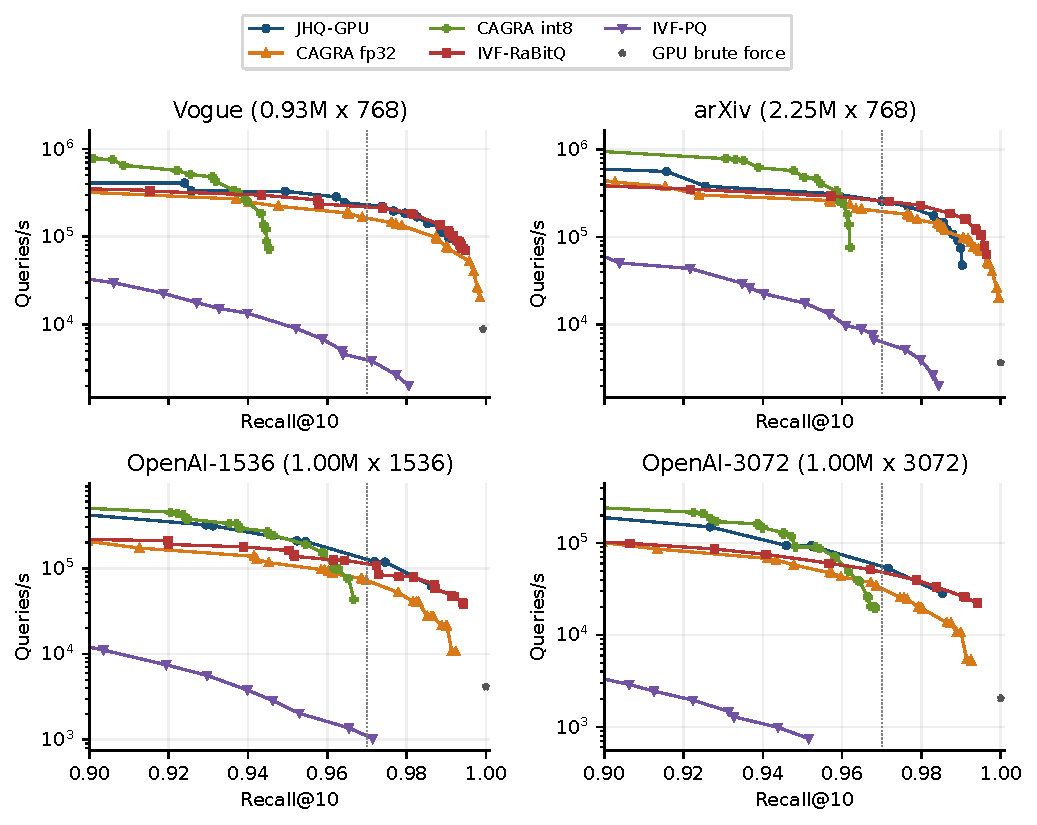
\includegraphics[width=\linewidth]{ch7/frontiers.pdf}
\caption[E1 recall--throughput frontiers]{Measured host-to-host recall--QPS frontiers on the four E1 datasets.
The displayed recall window begins at 0.90, with a vertical line at 0.97;
all baseline families,
including CAGRA int8, participate in frontier construction. Lines connect
measured points; throughput uses a logarithmic axis.}
\label{fig:7-frontiers}
\end{figure}

These curves are not memory-matched. Nine-bit RaBitQ has a nominal
$9d/8$ code budget comparable to JHQ, while its 4/8-bit arms use less.
\Cref{tab:4-bytes,sec:7-7} give representation costs and measured
allocations alongside this performance envelope.


\subsection{Matched recall and opposing operating regions}

\Cref{tab:7-matched} reports recall 0.97 using the interpolated and
qualifying-measured estimators defined in \cref{sec:3-4}.


\begin{table}[tbp]
\centering
\caption[Cross-system comparison at recall 0.97]{Recall 0.97 comparison. Each ratio is interpolated / measured;
values above one favour JHQ. JHQ kQPS is the interpolated estimate.
The small arXiv--RaBitQ difference changes direction with the estimator.}
\label{tab:7-matched}
\small\setlength{\tabcolsep}{4pt}
% Generated by scripts/build_ch7.py; do not edit numbers manually.
\begin{tabular}{@{}lrrr@{}}
\toprule
Dataset & JHQ kQPS & vs CAGRA fp32 & vs IVF-RaBitQ \\
\midrule
Vogue & 230.8 & 1.416 / 1.537 & 1.059 / 1.046 \\
arXiv & 258.6 & 1.317 / 1.422 & 0.996 / 1.015 \\
OpenAI-1536 & 126.7 & 1.747 / 2.294 & 1.130 / 1.111 \\
OpenAI-3072 & 55.9 & 1.747 / 2.088 & 1.157 / 1.346 \\
\bottomrule
\end{tabular}

\end{table}

At recall 0.97, JHQ's interpolated rate is $1.317$--$1.747\times$
CAGRA fp32's. It also leads IVF-RaBitQ on three datasets; arXiv is a
near tie whose direction changes with the estimator (\cref{tab:7-matched}).
Grid spacing matters: OpenAI-1536's CAGRA comparison is $1.747\times$
by interpolation and $2.294\times$ at qualifying measured points.

Vogue's lead depends on the grouped execution path. Replacing it by
$\gscan=0$ changes the recall-0.97 ratio against RaBitQ from $1.059$
to $0.933$ on the same batch-1,000 grid. Each pair fixes the index,
probes, budget and final outputs. This links RQ2 to RQ4 through the
integrated path, without isolating the shared bound alone.

The advantage changes with the recall target. CAGRA int8 is about
$1.20$--$1.98\times$ faster at 0.90--0.92 but has no qualifying point
at 0.97 in these grids. IVF-RaBitQ regains the lead at several targets
of 0.98 or above; CAGRA fp32 also leads on arXiv near 0.99.
\Cref{fig:7-frontiers} therefore supports a high-recall operating region,
with both the competitor's precision and measured coverage specified.

\subsection{Precision sensitivity on the OpenAI datasets}
\label{sec:7-precision}

Supplementary source inspection establishes that the E1 implementation
uses TF32 multiplication with FP32 accumulation for OpenAI rotation and
centroid GEMMs, despite FP32 input/storage and a misleading source comment
(\cref{sec:4-2}). The main E1 frontier remains the historical measurement
of that implementation. A separate FP32 variant changes the cuBLAS
math-mode switch and replays 37/39 OpenAI configurations at batch 1,000,
five rounds each. Execution order alternates between variants across
probe settings. Both reuse the same TF32-trained model; the intervention
changes add/query arithmetic, including database encoding and routing.
It is not a comparison of independently FP32-trained models.
\Cref{tab:7-precision} summarises the paired changes.

\par\medskip\noindent\begin{minipage}{\linewidth}
\centering\captionsetup{hypcap=false}
\captionof{table}[FP32 sensitivity at matched configurations]{FP32 sensitivity. QPS ratio is FP32/TF32 at equal configuration
(geometric mean); recall differences have the same direction. The last
two columns compare the FP32 frontier at recall 0.97 with archived E1
IVF-RaBitQ and CAGRA fp32 frontiers. Baselines were not remeasured.}
\label{tab:7-precision}
\scriptsize\setlength{\tabcolsep}{3pt}
\begin{tabular}{@{}lrrrrr@{}}
\toprule
Dataset & Pairs & QPS ratio & $\Delta$Recall & vs RaBitQ & vs CAGRA \\
\midrule
OpenAI-1536 & 37 & 0.953 & +0.0003--+0.0005 & 1.086 & 1.679 \\
OpenAI-3072 & 39 & 0.951 & +0.0000--+0.0003 & 1.079 & 1.629 \\
\bottomrule
\end{tabular}

\end{minipage}\par\medskip

At equal configuration, FP32 reduces throughput by about 5\% and increases
recall by 0--0.0005. At matched recall 0.97, its throughput is about 3\%
below the same-session TF32 frontier. It remains $1.086\times$ and
$1.079\times$ archived RaBitQ, and $1.679\times$ and $1.629\times$
archived CAGRA fp32. Same-session v69/RaBitQ ratios are 1.118/1.114,
versus historical 1.130/1.157. This separates the precision intervention
from session variation: the competitive direction persists, with smaller
margins, while the cross-session baseline comparison retains timing
uncertainty. The two precision variants' complete frontiers are shown in
\cref{fig:7-precision}.

\begin{figure}[tbp]
\centering
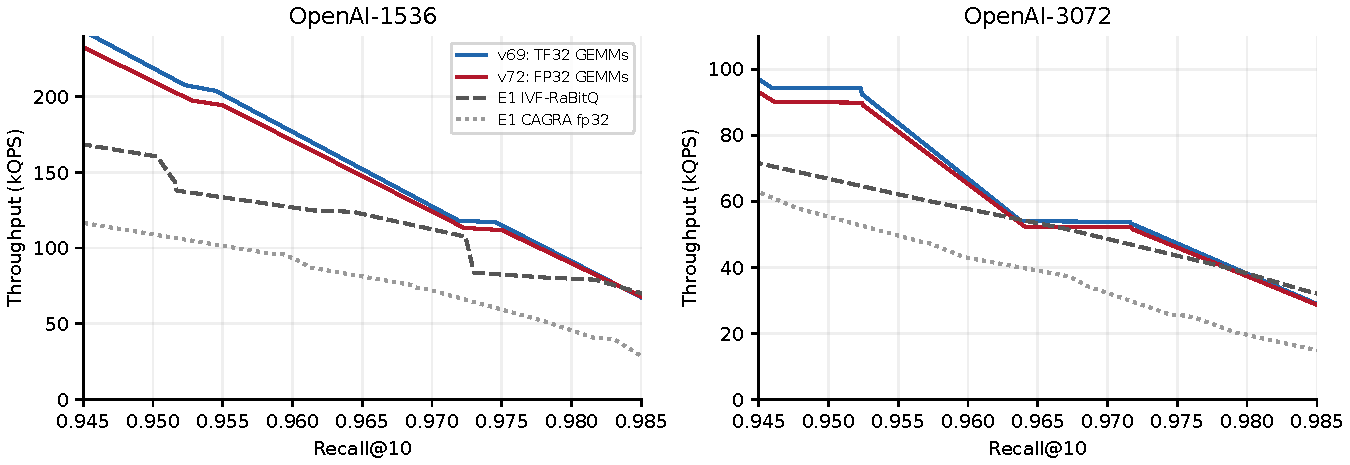
\includegraphics[width=\linewidth]{supplement/precision.pdf}
\caption[TF32 and FP32 precision frontiers]{Supplementary precision frontiers. Solid curves are same-session
JHQ variants; dashed/dotted baselines are historical E1 measurements.
All use the chapter's frontier and interpolation rules.}
\label{fig:7-precision}
\end{figure}


\subsection{Interpretation and comparison limits}

The OpenAI pair supplies a row-aligned embedding-width contrast from
Qdrant's DBpedia \texttt{text-embedding-3-large} corpus family
\cite{data_openai1536,data_openai3072}. The supplementary check compares
all 1,000 query rows and every 97th base row (10,299 rows): truncating
and renormalising the 3,072-dimensional vector gives cosine at least
0.9980 against its 1,536-dimensional counterpart, with median 1.000000.
GT top-10 overlap averages 9.046/10. This strongly supports matching row
order in the inspected exports; original entity-ID mappings were not
exported. Doubling dimension leaves the historical 0.97 CAGRA fp32
ratio at 1.747 in both datasets and changes the RaBitQ ratio from
1.130 to 1.157. The FP32 sensitivity likewise retains comparable
advantages. Dimension alone therefore does not explain the observed
advantage within this paired corpus/embedding contrast.

The four-dataset advantage co-varies with the 128-probe refinement
anchors: 4--8 for OpenAI, 64 for Vogue and 100 for arXiv
(the later FULL rule selects 200 there). These anchors are not the
matched-recall frontier parameters, so the association does not isolate
primary quality causally.

The interface, memory and compilation differences in \cref{sec:3-3}
remain relevant to small margins. \Cref{sec:7-8} examines their empirical
sensitivity.


\subsection{Small batches change the competitive region}
\label{sec:7-smallbatch}

T5 compares scheduled JHQ, CAGRA fp32/int8 and IVF-RaBitQ at batches
8/32 on the four E1 datasets. Five synchronous host-to-host rounds use
1,000/992 queries, respectively. Its 1,808 points include JHQ's one-block
control; IVF-PQ and brute force are outside this campaign.
\Cref{fig:7-smallbatch,tab:7-smallbatch} compare the resulting regions.

\suppressfloats[t]
\begin{figure}[htbp]
\centering
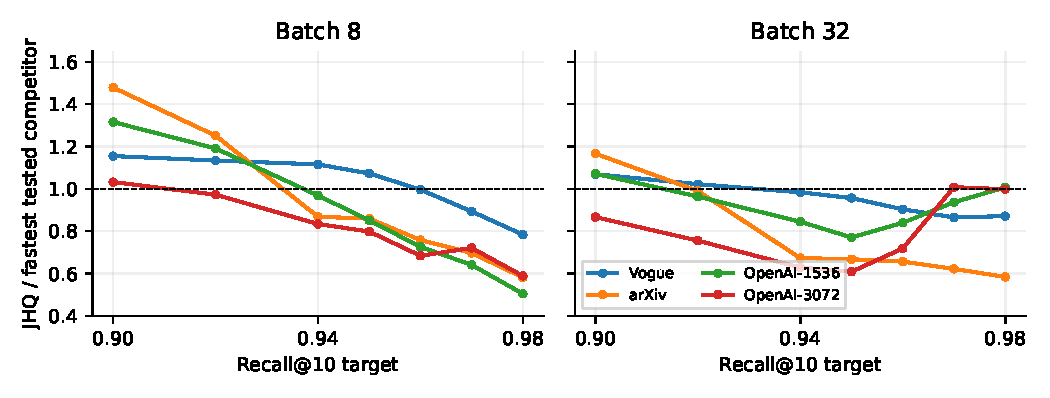
\includegraphics[width=\linewidth]{t4-t5/smallbatch.pdf}
\caption[Small-batch competitive regions]{T5 JHQ / fastest-competitor
QPS under interpolation with qualifying measured endpoints. Above one
favours JHQ. Strict measured thresholds are in \cref{tab:7-smallbatch}.}
\label{fig:7-smallbatch}
\end{figure}

\begin{table}[htbp]
\centering
\caption[Small-batch matched-recall ratios]{T5 QPS ratios:
interpolation with qualifying endpoints / strict measured threshold.
The fastest competitor is selected independently for each estimator;
higher-recall qualifying endpoints remain eligible without extrapolation.}
\label{tab:7-smallbatch}
\footnotesize\setlength{\tabcolsep}{4pt}
\begin{tabular}{@{}lrrrr@{}}
\toprule
Dataset & $b$ & $R=0.90$ & $R=0.95$ & $R=0.97$ \\
\midrule
Vogue & 8 & 1.155 / 1.091 & 1.073 / 0.980 & 0.893 / 0.854 \\
Vogue & 32 & 1.069 / 0.997 & 0.956 / 0.895 & 0.865 / 0.839 \\
arXiv & 8 & 1.479 / 1.454 & 0.859 / 0.851 & 0.697 / 0.698 \\
arXiv & 32 & 1.166 / 1.148 & 0.667 / 0.661 & 0.622 / 0.582 \\
OpenAI-1536 & 8 & 1.316 / 1.131 & 0.851 / 0.825 & 0.641 / 0.620 \\
OpenAI-1536 & 32 & 1.071 / 0.915 & 0.770 / 0.752 & 0.937 / 0.914 \\
OpenAI-3072 & 8 & 1.032 / 0.953 & 0.798 / 0.798 & 0.721 / 0.702 \\
OpenAI-3072 & 32 & 0.866 / 0.734 & 0.608 / 0.771 & 1.008 / 1.351 \\
\bottomrule
\end{tabular}

\end{table}

At recall 0.97 and batch 8, CAGRA fp32 leads on all four datasets under
both estimators: interpolated JHQ ratios are 0.641--0.893. At batch 32,
these ratios are 0.622--1.008, with OpenAI-3072 close under interpolation
but favourable to JHQ under the measured threshold. At recall 0.95,
Vogue's batch-8 lead likewise appears only under interpolation. Grid
resolution therefore matters to borderline rankings.

Lower-recall comparisons must retain competitors whose fastest frontier
point already exceeds the target.
At 0.90, corrected interpolated ratios are 1.032--1.479 at batch 8 and
0.866--1.166 at batch 32; the strict measured estimator gives three
and one JHQ wins, respectively. Omitting qualifying endpoints would
overstate these low-recall leads.
Scheduling is still useful: at recall 0.95 its interpolated gain over
one block is 1.7--3.3$\times$. An internal execution gain therefore need
not produce a cross-system lead.

Null-call medians by dataset, method and batch span 0.012--0.072\,ms;
this overhead remains in search timing. CAGRA uses Python bindings, while JHQ/RaBitQ use C++;
warm-up policies also differ. Protocol and grid details are in \cref{sec:a-t4-t5}. E1's full-batch
high-recall leads do not generalise to these small batches.


\section{Cartesian LUT, Packed Loads and Lane Refinement}
\label{sec:7-3}

The RQ2 ablations measure both kernel and application effects.

\subsection{Exact table factorization and its throughput consequence}

The LUT ablation tests the cost model in \cref{sec:5-2} and FP32 ranking
effects.


\Cref{fig:7-lut} compares Cartesian table grouping on six datasets,
probe counts 8/32/128/512,
fixed $\alpha=100$, and $\glut\in\{1,2,4,8\}$. Each arm has five timing
rounds; batch size is 1,000 except Stella's 999 queries. Two groups have
the highest median throughput in 22 of 24 cells. The exceptions are
arXiv at 128 probes, where one group is about 0.23\% faster, and
OpenAI-3072 at eight probes, where four groups are about 0.84\% faster.
These narrow differences are best treated as near ties. The newer count
is 22/24, rather than the historical ADC paper's 23/24.
In the specific two-group versus one-group comparison, two groups win
23/24 cells; each dataset's four-probe geometric-mean ratio exceeds one
(1.021--1.318). This supports the choice across the tested workloads
without treating configurations sharing an index as independent trials.

\begin{figure}[tbp]
\centering
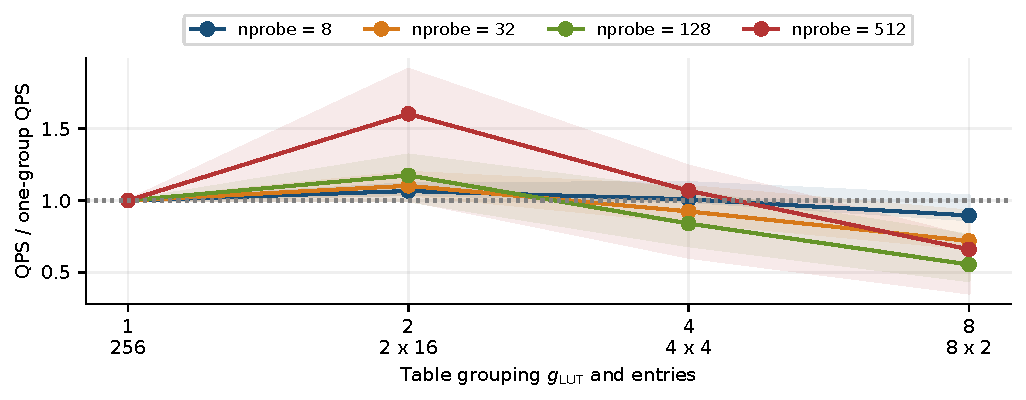
\includegraphics[width=\linewidth]{ch7/lutgroups.pdf}
\caption[Cartesian lookup-table grouping]{Cartesian table grouping at fixed $\alpha=100$ (v71).
Group counts describe $\glut$, not parallel scan groups. Curves are medians
of per-dataset QPS ratios to the one-group arm; shading shows their range.}
\label{fig:7-lut}
\end{figure}

The two-group/one-group ratio ranges from $0.998$ to $1.914$.
Four and eight groups each store 16 entries but require more lookups
and additions. These arms show that smaller tables need not improve
throughput; occupancy and instruction costs were not isolated. The maximum
reported recall spread within any four-arm cell is $10^{-4}$.
At 128 probes and $\alpha=100$, T4 compares identical candidates on
Vogue, arXiv and OpenAI-3072. Full versus $16+16$ tables differ in
22.6--26.1\% of candidate-score bit patterns, with maximum relative error
$4.53\times10^{-7}$. Across all forms, 20.5--29.4\% differ, with maximum
relative error $4.64\times10^{-7}$. Vogue has 2--4/256 final-ID
differences, while arXiv/OpenAI have none. Unchanged primary survivor
sets can still produce different final IDs because the rounded primary
score enters refinement (\cref{sec:a-t4-t5}).


\subsection{Packed access and cooperative residual scoring}

The historical packing experiment compares byte-oriented and word-oriented
access while holding the dataset, probe count and table grouping fixed.
Across six datasets, four probe counts and $\glut\in\{1,2\}$, the 48
pairs yield throughput ratios from $1.012$ to $1.658$, with maximum recall
difference $10^{-4}$. Gains are generally smaller at eight probes and
larger at 512. Both alternatives already use a subspace-major layout;
this experiment supports packed access, not a claim that a physical
transpose alone produced the improvement. Each arm has one reported
aggregate rate, so this older evidence has weaker uncertainty information
than the five-round v71 sweep.

\Cref{fig:7-packing-refinement,tab:7-refinement} then separate wider loads
from lane cooperation in residual refinement. L0 is the original scalar
path; L1 changes the load path without distributing a candidate across
multiple lanes; L16 assigns 16 lanes to a candidate. The same process
rotates arm order across five timing rounds, with three search calls per
arm per round. For the twelve ordinary configurations, L16 improves
end-to-end throughput by $1.015$--$1.789\times$. An additional arXiv
configuration at $\alpha=200$, explicitly a high-budget control, reaches
$2.383\times$; it is not the gain range of the ordinary selected budgets.

\begin{figure}[tbp]
\centering
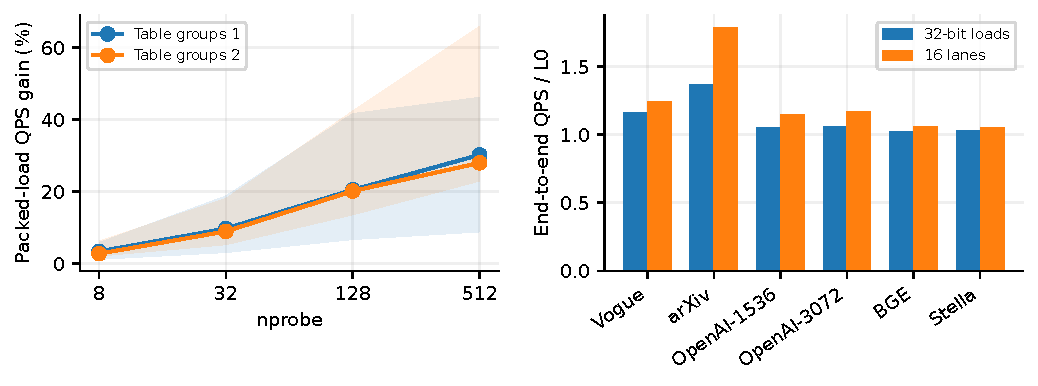
\includegraphics[width=\linewidth]{ch7/packing_refinement.pdf}
\caption[Packed access and refinement controls]{Packing and refinement controls. Left: median packed-load QPS
 gain across six datasets, with shaded minimum--maximum ranges, for each
 table grouping and probe count. Right: measured load-only and 16-lane
 end-to-end gains at 128 probes and the ordinary dataset-specific budgets.
 These panels come from different experiment families.}
\label{fig:7-packing-refinement}
\end{figure}

\begin{table}[tbp]
\centering
\caption[Refinement gains at 128 probes]{Refinement at 128 probes. Ratios are paired end-to-end gains over
 L0, except the last column, which is the profiled refinement-kernel gain.
 The kernel and application gains must not be interchanged.}
\label{tab:7-refinement}
\small\setlength{\tabcolsep}{4pt}
% Generated by scripts/build_ch7.py; do not edit numbers manually.
\begin{tabular}{@{}lrrrr@{}}
\toprule
Dataset & $\alpha$ & $L1/L0$ QPS & $L16/L0$ QPS & Kernel gain \\
\midrule
arXiv & 100 & 1.368 & 1.789 & 5.97 \\
BGE & 32 & 1.026 & 1.062 & 1.97 \\
OpenAI-1536 & 8 & 1.055 & 1.145 & 3.34 \\
OpenAI-3072 & 4 & 1.063 & 1.171 & 8.81 \\
Stella & 16 & 1.030 & 1.053 & 2.66 \\
Vogue & 64 & 1.161 & 1.240 & 3.72 \\
\bottomrule
\end{tabular}

\end{table}

The load-only control is bit-identical to L0 in the tested cases, yet
already improves arXiv throughput by $1.368\times$. Lane cooperation adds
a larger reduction in refinement time. On arXiv at $\alpha=100$, the
profiled refinement kernel falls from 4,277.5 to 716.8\,$\mu$s, a
$5.97\times$ gain, while total throughput improves $1.789\times$.
OpenAI-3072's refinement kernel improves $8.81\times$, but total throughput
improves $1.171\times$. The remaining routing, screening, selection and
transfer costs limit the application gain.

A quantitative Amdahl check uses the refinement kernel's baseline time
as a fraction $f$ of host-to-host baseline latency and its kernel speedup
$s$, giving $1/(1-f+f/s)$ if the remaining time is unchanged. The fractions
are approximately 0.529 on arXiv and 0.168 on OpenAI-3072, producing
estimates of $1.787\times$ and $1.175\times$, close to the measured
$1.789\times$ and $1.171\times$. These combine separate kernel-profile
and wall-time measurements and are explanatory estimates.

Cooperative reductions alter floating-point addition order. The tested
multi-lane variants have very small distance differences, with maximum
reported relative error about $1.6\times10^{-6}$, and occasional changes
near ranking boundaries. Sanitizer checks cover the recorded refinement
and top-$k$ kernels on small query subsets. These checks and numerical
tolerances delimit the evidence; multi-lane scoring is not universally
bit-identical.

\section{Global Top-c, Shared Bound and Probe Correctness/Ablation}
\label{sec:7-4}

The representation checks in \cref{sec:4-6} concern the stored index;
this section evaluates query selection and its cost.


\subsection{Strict CPU reference for computed-score selection}
\label{sec:7-strict-selection}

The supplementary T4 campaign sorts every visited candidate on the CPU
under $(\primarydist,\mathrm{position})$, using GPU-produced FP32 scores.
Its diagnostic exporter follows the packed scan layout and accumulation
order; exported scores match all returned valid primary scores bit for
bit. Source comparison confirms that the diagnostic version changes only
export, relative to the table-sweep implementation.
Vogue, arXiv and OpenAI-3072 are tested at 1/8/128 probes,
$\alpha\in\{4,100,200\}$, $\gscan\in\{0,1,2,4,8\}$ and both shared-bound
settings: 270 configurations of 256 queries, or 69,120 query instances
(\cref{tab:7-strict-selection}).

\suppressfloats[t]
\begin{table}[htbp]
\centering
\caption[Strict computed-score selection checks]{T4 CPU-reference checks.
Set and order equality use the complete primary key. Valid count checks
$\min(c,n_c)$ survivors; final equality sorts retained computed refined
scores by $(\refineddist,\mathrm{ID})$, including their FP32 bits. Counts
are query instances, with queries reused across configurations.}
\label{tab:7-strict-selection}
\footnotesize\setlength{\tabcolsep}{3pt}
\begin{tabular}{@{}lrrrrr@{}}
\toprule
Path & Queries & Set / order exact & Tie-only & Valid count & Final exact \\
\midrule
$\gscan\geq1$ & 55,296 & 55,296 / 55,296 & 0 & 55,296 & 55,296 \\
$\gscan=0$ & 13,824 & 13,768 / 8,758 & 56 & 13,824 & 13,824 \\
\bottomrule
\end{tabular}

\end{table}

All 55,296 grouped instances match the complete-key reference in order.
The one-block path satisfies the distance preorder in all 13,824 instances;
its 56 set differences are exclusively cutoff ties. There are 19,120
underfull instances with the correct number of valid survivors, and all
69,120 final selections match the retained-score reference.
This directly tests the stage contracts of
\cref{lem:5-buffer,prop:5-local-coverage,prop:5-shared-bound}.
The earlier 64 scan comparisons and 48 shared-bound comparisons provide
separate paired-implementation evidence; archived sanitizer runs cover
smaller subsets. Export and retention details are in \cref{sec:a-t4-t5}.


\subsection{Shared bounds preserve the selection target}

\Cref{prop:5-shared-bound} establishes the selection guarantee. The
paired experiment measures the work saved by sharing that bound.


Across four workloads and four batch sizes, all 48 shared-bound versus
independent-bound comparisons agree on primary and final outputs.
Five-round paired throughput ratios span $0.994$--$1.562\times$.
On arXiv at $\alpha=200$, batch 1,000 and eight groups, the paired
profile reduces merge time from about 2,629 to 471\,$\mu$s and scan
from 7,968 to 5,513\,$\mu$s. Sharing therefore reduces intermediate work
in suitable workloads, with small regressions elsewhere.

The rejected static-quota design faces concentrated winners: the first
candidate group holds 46--81\% of global survivors in the pilot workloads.
Equal quotas would require a correctness fallback; calibrated unequal
quotas leave the dominant group on the critical path. These observations
motivate shared bounds within that pilot's scope.

\subsection{Exact probe selection and the limits of pipeline identity}

Once screening becomes faster, IVF probe selection becomes a larger
fraction of small-batch time. The radix probe primitive (v69) changes how the
smallest computed centroid scores are selected while retaining the
preceding score arithmetic. On OpenAI this includes TF32 GEMMs
(\cref{sec:7-precision}).
Its synthetic checker covers 1,792 cases and reports zero failures.
Checks of the real arXiv, Vogue and OpenAI-3072 workloads find identical
probe identifiers and identical primary top-$c$ positions and distances
for all 1,000 queries.

\begin{table}[tbp]
\centering
\caption[Probe-selection throughput ratios]{v69/v65 end-to-end throughput ratios for the exact computed-score probe
 change. Each workload--batch comparison has ten timing rounds per binary,
 collected in alternating runs. Values above one favour v69.}
\label{tab:7-probe}
\small
% Generated by scripts/build_ch7.py; do not edit numbers manually.
\begin{tabular}{@{}lrrrr@{}}
\toprule
Dataset & Batch 8 & 32 & 256 & 1,000 \\
\midrule
arXiv & 1.074 & 1.063 & 1.035 & 1.034 \\
Vogue & 1.109 & 1.103 & 1.052 & 1.041 \\
OpenAI-3072 & 1.167 & 1.117 & 1.055 & 1.050 \\
\bottomrule
\end{tabular}

\end{table}

\Cref{tab:7-probe} shows end-to-end improvements of $1.034$--$1.167\times$.
At batch 8, the profiled probe stage falls from 56.5 to 22.6\,$\mu$s
on arXiv, 52.7 to 14.7\,$\mu$s on Vogue, and 77.8 to 16.7\,$\mu$s
on OpenAI-3072. The unchanged stages limit full-batch gains. These
within-family ratios have different baselines from the preceding ablations.

On Vogue, the probe/primary dump is
byte-identical across the two binaries for all 1,000 queries in the
one-group, batch-8 test, yet final recall is 0.9642 versus 0.9644. The
same baseline binary also changes from 0.9642 in the identity run to
0.9644 in each of its two timing runs. The variation therefore also
occurs without the probe change and lies after primary selection in the
dump-controlled case. Its root cause remains unresolved. Scheduled and
one-block outputs are bit-identical within each checked process; dump
coverage is in \cref{app:reproducibility}.

Finally, the optional v70 FP16 experiment is a separate approximation.
Its probe sets match the v69 reference on 936/1,000 arXiv queries, 979/1,000
Vogue queries and 998/1,000 OpenAI-3072 queries, with very high mean
set overlap. High overlap and small recall changes do not make the
primitive exact. Those results are excluded from the main E1 frontier
and from the exact-probe claim.

\section{Held-out Budget Quality, Throughput and Payback}
\label{sec:7-5}

RQ3 compares the policy of \cref{ch:refinement} with fixed
$\alpha=100$ and the stronger universal control $\alpha=64$.

\subsection{Unlabelled selection and a labelled diagnostic oracle}

The six datasets are tested at 128 and 512 probes with the fixed,
sampled, FULL, enumeration and oracle controls in \cref{sec:6-4}.
The disjoint pools and 64 draws per sample size follow \cref{sec:3-2}.


All rule variants use \cref{eq:6-agreement} with $k=10$ and $\epsilon=1$.
FULL uses all calibration queries; the diagnostic oracle uses held-out
labels (\cref{tab:6-controls}).


\subsection{Full-pool calibration as the quality-first working point}

Full-pool calibration uses all 500 calibration queries once per cell.
Its selected arms meet the held-out $10^{-3}$ loss target in 12/12 cells;
the largest observed loss is 0.0006. Their rates are 0.908--1.000 of the
GT oracle's, and calibration costs 9.5--60.3\,ms. The geometric-mean
rate ratio to fixed 100 is $1.111\times$, or $1.193\times$ over the ten
cells where fixed 100 also meets the target. \Cref{tab:7-budget-full}
shows the complete comparison. Against fixed 64, full-pool selection is
faster in six cells, equal in two and slower in four: its main advantage
is the observed coverage of all twelve quality targets.

These cells favour FULL for quality coverage and $S=128$ for lower
calibration cost, within the statistical scope of \cref{sec:6-2}.


\begin{table}[tbp]
\centering
\caption[Full-pool budget calibration]{Full-pool calibration ($S=500$). Loss is relative to the best
measured held-out recall; rates are kQPS from the selected fixed arm.
``Cal.'' is one full-pool calibration call per cell, not a repeated
stream timing. Held-out counts are 500, or 499 for Stella.}
\label{tab:7-budget-full}
\footnotesize\setlength{\tabcolsep}{3pt}
% Generated by scripts/build_ch7.py; do not edit numbers manually.
\begin{tabular}{@{}lrrrrrrr@{}}
\toprule
Dataset & Probe & $\alpha_{\rm full}$ & Loss & $Q_{\rm full}$ & vs 100 & vs oracle & Cal. ms \\
\midrule
Vogue & 128 & 100 & 0.0000 & 202.9 & 1.000 & 0.908 & 10.1 \\
arXiv & 128 & 200 & 0.0000 & 151.5 & 0.728 & 1.000 & 10.0 \\
OpenAI-1536 & 128 & 8 & 0.0000 & 267.7 & 1.599 & 1.000 & 9.5 \\
OpenAI-3072 & 128 & 4 & 0.0000 & 145.0 & 1.691 & 1.000 & 17.1 \\
BGE & 128 & 64 & 0.0006 & 124.9 & 1.075 & 0.932 & 17.1 \\
Stella & 128 & 16 & 0.0006 & 110.4 & 1.153 & 1.000 & 20.6 \\
Vogue & 512 & 100 & 0.0002 & 100.1 & 1.000 & 0.969 & 20.9 \\
arXiv & 512 & 200 & 0.0000 & 69.0 & 0.831 & 1.000 & 25.1 \\
OpenAI-1536 & 512 & 8 & 0.0000 & 114.9 & 1.326 & 1.000 & 21.8 \\
OpenAI-3072 & 512 & 4 & 0.0002 & 52.1 & 1.219 & 0.977 & 40.5 \\
BGE & 512 & 64 & 0.0006 & 50.8 & 1.033 & 1.000 & 42.3 \\
Stella & 512 & 16 & 0.0006 & 36.0 & 1.041 & 1.000 & 60.3 \\
\bottomrule
\end{tabular}

\end{table}

\subsection{Lower-cost sampling and its quality risk}

\Cref{tab:7-budget-quality} reports the $S=128$ result. The median selected
budget matches the oracle budget in ten of twelve cells; it differs on
arXiv at 128 probes and OpenAI-3072 at 512. The selected budgets span
4--200, indicating substantial workload dependence. Median budget and
mean recall need not describe one arm. The latter is reconstructed from
printed best recall minus mean loss and is approximate at four decimals.

\begin{table}[tbp]
\centering
\caption[Sampled-budget held-out quality]{Held-out quality at $S=128$. Rule $\alpha$ is the median across
64 draws; oracle $\alpha$ uses held-out labels. $\overline R_{\rm rule}$
is reconstructed mean recall. ``Losses'' counts draws with recall loss
$>10^{-3}$ relative to the best tested held-out recall; $L_{95}$ is the
logged lower-order 95th-percentile loss estimate. $R_{100}$ is
fixed-budget recall.}
\label{tab:7-budget-quality}
\small\setlength{\tabcolsep}{3pt}
% Generated by scripts/build_ch7.py; do not edit numbers manually.
\begin{tabular}{@{}lrrrrrr@{}}
\toprule
Dataset & Probe & $\alpha$: rule/oracle & $R_{100}$ & $\overline{R}_{\rm rule}$ & Losses & $L_{95}$ \\
\midrule
Vogue & 128 & 64 / 64 & 0.9680 & 0.9677 & 5/64 & 0.0022 \\
arXiv & 128 & 100 / 200 & 0.9748 & 0.9751 & 40/64 & 0.0024 \\
OpenAI-1536 & 128 & 8 / 8 & 0.9280 & 0.9279 & 4/64 & 0.0000 \\
OpenAI-3072 & 128 & 4 / 4 & 0.9252 & 0.9252 & 0/64 & 0.0000 \\
BGE & 128 & 32 / 32 & 0.9198 & 0.9190 & 1/64 & 0.0008 \\
Stella & 128 & 16 / 16 & 0.9892 & 0.9884 & 6/64 & 0.0030 \\
Vogue & 512 & 64 / 64 & 0.9916 & 0.9915 & 2/64 & 0.0002 \\
arXiv & 512 & 200 / 200 & 0.9878 & 0.9885 & 32/64 & 0.0016 \\
OpenAI-1536 & 512 & 8 / 8 & 0.9740 & 0.9738 & 4/64 & 0.0000 \\
OpenAI-3072 & 512 & 4 / 8 & 0.9704 & 0.9702 & 0/64 & 0.0002 \\
BGE & 512 & 64 / 64 & 0.9670 & 0.9661 & 24/64 & 0.0014 \\
Stella & 512 & 16 / 16 & 0.9954 & 0.9945 & 7/64 & 0.0030 \\
\bottomrule
\end{tabular}

\end{table}

ArXiv exposes the sampling risk: 40/64 draws at 128 probes and 32/64
at 512 exceed the $10^{-3}$ loss threshold, despite mean loss 0.0009
in both cells. Fixed 100 itself loses 0.0012/0.0016, so improvement
over that default coexists with failure against the stronger target.
Other tails are in \cref{tab:7-budget-quality}: BGE/512 has 24/64
crossings and $L_{95}=0.0014$; Stella has $L_{95}=0.0030$ at both
probe depths, while OpenAI-3072 has no observed crossings.
Under the percentile convention in \cref{sec:a-budget-contract},
four nonzero losses can coexist with $L_{95}=0$, as on OpenAI-1536.

\begin{figure}[tbp]
\centering
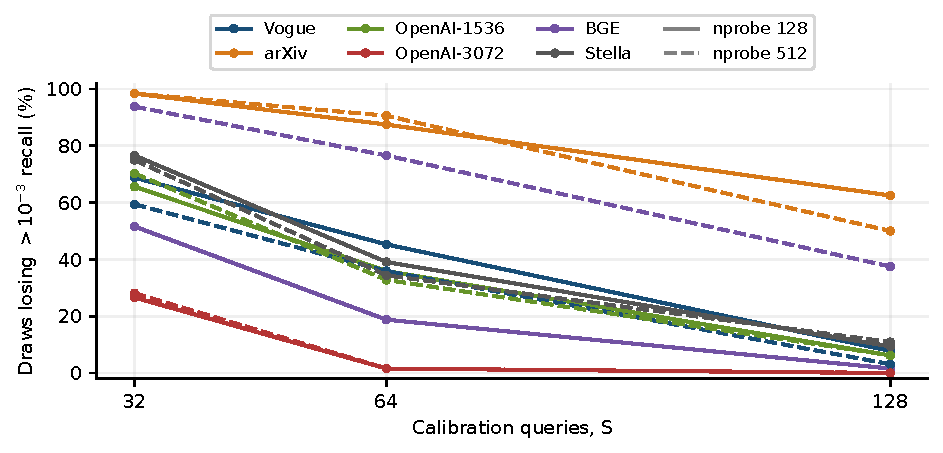
\includegraphics[width=0.82\linewidth]{ch7/budget_risk.pdf}
\caption[Held-out risk across sample sizes]{Held-out risk across sample sizes. The vertical axis is the
percentage of calibration draws losing more than $10^{-3}$ held-out recall
relative to the best tested budget. Increasing $S$ also tightens the allowed
slot-disagreement fraction because \cref{eq:6-agreement} keeps threshold one.}
\label{fig:7-budget-risk}
\end{figure}

Increasing $S$ tightens the normalised allowance $1/(10S)$ as well
as changing sample coverage (\cref{fig:7-budget-risk}).
The grouped-path guarantee covers 2,176/2,304 sampled draws;
the remaining 128 distance-only cases are empirical checks
(\cref{cor:6-grouped-calibration}). Enumeration and FULL verification
are reported in \cref{sec:7-budget-trace}.

Fixed 64 and fixed 100 each meet the diagnostic quality target in 10/12
cells; fixed 200 meets it in all twelve. FULL selects 100 on Vogue
where the fastest qualifying oracle arm is 64: minimum reference
disagreement and maximum quality-constrained throughput are different
objectives. The observed low-budget timing plateau reinforces this
distinction.

\subsection{Estimated throughput and calibration economics}

Using the mean selected-arm QPS estimate specified in
\cref{sec:a-budget-contract}, $S=128$ improves over fixed $\alpha=100$
in ten cells by $1.028$--$1.691\times$. On arXiv the ratios are 0.908
and 0.917: mean recall improves, but throughput falls, giving no
throughput payback.


Against fixed 64, selected-arm QPS wins in 9/12 cells with geometric
mean $1.054\times$ and range $0.821$--$1.367\times$; OpenAI gains are
$1.052$--$1.367\times$. Both fixed controls fail the two arXiv quality
targets. These are consequently joint quality/time comparisons, rather
than uniform speedups over an acceptable fixed budget.

\begin{table}[tbp]
\centering
\caption[Sampled-calibration economics]{Calibration economics, $S=128$. Rates are kQPS and rule rate is
mean selected-arm QPS. Ratios compare with fixed 100 and fixed 64.
The ``Batches'' column gives payback relative to fixed 100 using 500
queries, or 499 for Stella; ``Never'' denotes no throughput payback.
The quality column separately marks whether fixed 100 meets the
held-out loss target.}
\label{tab:7-budget-cost}
\footnotesize\setlength{\tabcolsep}{3pt}
% Generated by scripts/build_ch7.py; do not edit numbers manually.
\begin{tabular}{@{}lrrrrrr@{}}
\toprule
Dataset & Probe & $Q_{100}$ & $\overline Q_{\rm rule}$ & Ratio & Cal. ms & Batches \\
\midrule
Vogue & 128 & 202.9 & 224.4 & 1.106 & 4.0 & 17.0 \\
arXiv & 128 & 207.9 & 188.8 & 0.908 & 4.2 & Never \\
OpenAI-1536 & 128 & 167.5 & 268.5 & 1.603 & 3.9 & 3.5 \\
OpenAI-3072 & 128 & 85.7 & 145.0 & 1.691 & 5.7 & 2.4 \\
BGE & 128 & 116.2 & 131.2 & 1.130 & 6.5 & 13.2 \\
Stella & 128 & 95.7 & 110.3 & 1.153 & 7.5 & 10.8 \\
Vogue & 512 & 100.1 & 102.9 & 1.028 & 7.5 & 55.4 \\
arXiv & 512 & 83.1 & 76.2 & 0.917 & 9.7 & Never \\
OpenAI-1536 & 512 & 86.6 & 115.0 & 1.327 & 8.8 & 6.2 \\
OpenAI-3072 & 512 & 42.8 & 52.1 & 1.219 & 13.1 & 6.2 \\
BGE & 512 & 49.2 & 51.1 & 1.039 & 15.8 & 41.2 \\
Stella & 512 & 34.6 & 36.0 & 1.041 & 21.3 & 37.1 \\
\bottomrule
\end{tabular}

\end{table}

Calibration costs 3.9--21.3\,ms. Applying \cref{eq:6-payback} gives
the batch estimates in \cref{tab:7-budget-cost}, subject to the
stationary-reuse and inverse-mean-rate assumptions of \cref{sec:6-5}.
The largest positive $S=128$ payback estimates correspond to
0.54/2.72\,s against fixed 100/64; FULL's corresponding maxima are
1.52/2.25\,s. ArXiv's fixed controls miss the quality target, so their
timing ratios are diagnostic. Direct reuse below tests net cost with
quality reported alongside time.

\subsection{Complete decision traces and finite-pool risk}
\label{sec:7-budget-trace}

All 2,304 sampled curves are monotone and bisection selects the
enumerated minimum; the twelve FULL calls also pass both checks.
Summing full-pool per-query counts over recorded sample IDs reproduces
all 18,432 grid counts, supporting \cref{eq:6-finite-pool} on these
subsets. This aggregate check does not establish per-query invariance
for arbitrary subsets or positions. The structural grouped-path
guarantee and distance-only exceptions remain those of
\cref{sec:6-3}.

At $S=128$, maxima reach 0.0050 for arXiv/512 and 0.0046 for BGE/512;
at $S=32$ the largest is 0.0294. A low mean loss therefore coexists
with occasional materially worse chosen budgets. FULL's maximum across
the twelve cells remains 0.0006.

For arXiv/128, predicted crossings at $S=32,64,128$ are
0.965/0.875/0.620, versus 0.984/0.875/0.625 observed
(\cref{fig:7-finite-pool}). The largest discrepancy among 36 comparisons
is 0.144 on BGE/512 at $S=128$ (0.519 predicted, 0.375 observed).
Prediction conditions on stable query counts and uses held-out fixed-arm
quality to map accepted budgets to GT loss; the agreement decision itself
uses no labels.

\begin{figure}[tbp]
\centering
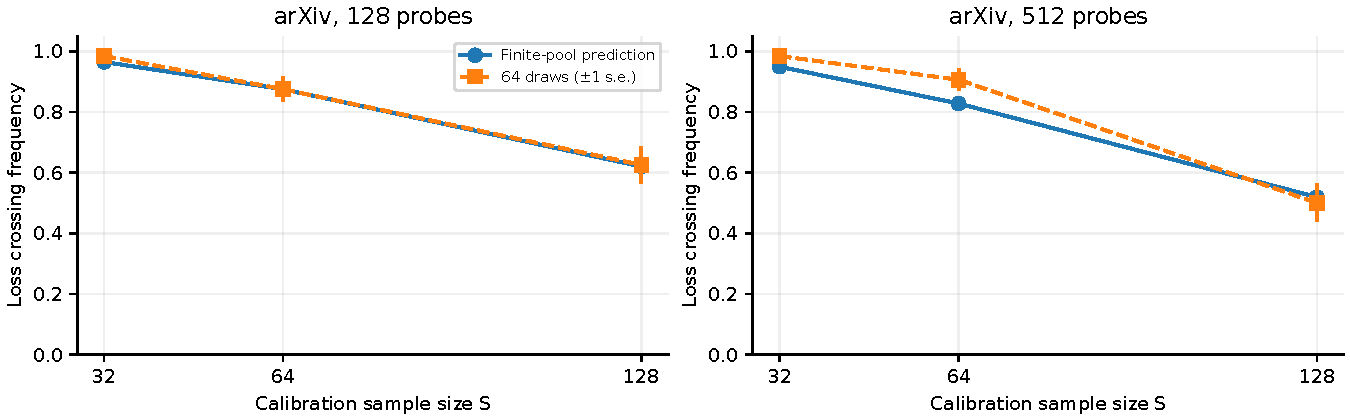
\includegraphics[width=\linewidth]{supplement/finite-pool.pdf}
\caption[Finite-pool risk prediction and observation]{Finite-pool prediction and observed arXiv loss crossings. Bars
show one estimated standard error over 64 independently drawn subsets
conditional on the fixed pool, not uncertainty over future workloads.}
\label{fig:7-finite-pool}
\end{figure}

Ten alternating repetitions resolve the apparent small-budget speed
inversion into a low-budget timing plateau. This observation does not
impose monotone runtime across all budgets and resource transitions.

\subsection{Direct calibration-plus-reuse measurement}
\label{sec:7-stream-cost}

Four cells compare fixed 64/100 with sampled and FULL calibration
over five rotated-policy rounds and 500 held-out batches. The timer
includes gathering, calibration, budget installation and first-batch graph
setup; construction, warm-up and scan calibration are excluded.
The same query pool is replayed (\cref{tab:7-stream-cost}).

\par\medskip\noindent\begin{minipage}{\linewidth}
\centering\captionsetup{hypcap=false}
\captionof{table}[Direct costs for 500 reuse batches]{Direct total milliseconds for 500 reuse batches, averaged over
five rounds, including budget calibration for sampled and FULL policies.
Each batch has 500 queries. Quality is discussed with the timing results.}
\label{tab:7-stream-cost}
\footnotesize\setlength{\tabcolsep}{4pt}
\begin{tabular}{@{}lrrrr@{}}
\toprule
Dataset/probes & Fixed 100 & Fixed 64 & Rule $S=128$ & FULL \\
\midrule
arXiv/128 & 1224 & 1102 & 1291 & 1680 \\
OpenAI-1536/128 & 1491 & 1264 & 852 & 860 \\
OpenAI-3072/128 & 2757 & 2160 & 1769 & 1783 \\
BGE/512 & 5185 & 5018 & 4921 & 5062 \\
\bottomrule
\end{tabular}

\end{minipage}\par\medskip

On OpenAI-3072/128, the sampled policy selects 4 in every round and
reduces total time from 2,757 to 1,769\,ms against fixed 100, about
36\%, at the same measured recall 0.9252. FULL selects the same budget
and takes 1,783\,ms including its larger calibration cost. On
OpenAI-1536/128, FULL takes 860 versus 1,491\,ms at the same recall
0.9280; the sampled policy averages 852\,ms and 0.9276 recall.

Measured mean cumulative savings first appear at 4/6 batches on
OpenAI-1536 and 4/9 on OpenAI-3072 against fixed 100/64
(\cref{fig:7-stream-cost}); fractional steady-rate fits are separate
model estimates. BGE/512 trades lower time for lower mean recall:
4,921 versus 5,185\,ms and 0.9658 versus 0.9670 for sampled/fixed 100.
FULL reaches 0.9664 at 5,062\,ms. ArXiv's FULL policy selects 200 for
quality and is slower than fixed 100/64, which miss the target.
Calibration's benefit therefore depends jointly on quality and total
reuse cost.

\begin{figure}[tbp]
\centering
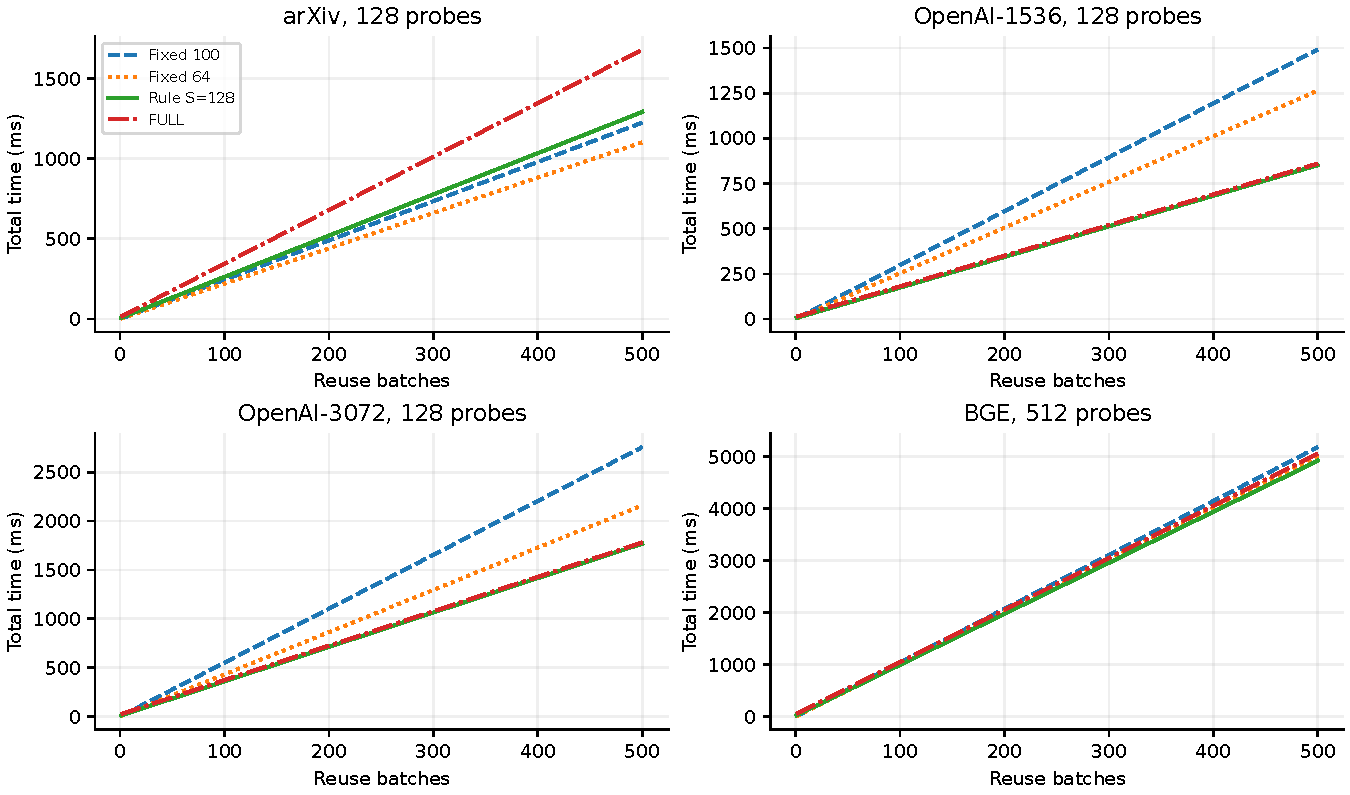
\includegraphics[width=\linewidth]{supplement/stream-cost.pdf}
\caption[Direct cumulative calibrated-reuse time]{Direct mean cumulative time, including budget calibration and
first-batch setup. Each curve replays one fixed held-out query pool.
Policies can have different recall; timings alone are not a quality-matched
ranking. Dataset/probe settings match \cref{tab:7-stream-cost}.}
\label{fig:7-stream-cost}
\end{figure}


\section{Batch Regimes, G Scheduling and Workload Skew}
\label{sec:7-6}

This section answers the performance-regime part of RQ2: when additional
scan groups supply useful parallelism, and when their extra work dominates.

\subsection{Parallelism versus repeated selection work}

For a fixed workload and timing boundary, separate scan, merge and
remaining execution time:
\begin{equation}
 \begin{aligned}
 T^{(g)}&=T_{\rm scan}^{(g)}+T_{\rm merge}^{(g)}+T_{\rm other}^{(g)},\\
 \Delta T(g)&=T^{(g)}-T^{(0)},\qquad
 T^{(g)}<T^{(0)}\iff\Delta T(g)<0.
 \end{aligned}
 \label{eq:7-group-cost}
\end{equation}
Here $g=0$ denotes the query-centric implementation and $g>0$ a grouped
path. The three time categories are disjoint: staging and local
selection already included in scan time are not charged again.
This is an accounting identity, not an analytical latency predictor.

At batch 8, one block per query exposes only eight blocks on 170 SMs.
Eight scan groups improve end-to-end throughput by $2.06$--$2.76\times$.
For example, arXiv's scan falls from 849 to 216\,$\mu$s while merging
adds 16.7\,$\mu$s. At batch 1,000, arXiv with $\alpha=200$ instead
increases scan time from 3,530 to 7,652\,$\mu$s and adds
2,624\,$\mu$s of merging; the independent-bound path reaches only
about $0.46\times$ its one-block throughput. Extra parallelism repays
its duplicated work in the first regime and loses in the second.
Shared bounds reduce work without removing this regime change.

\begin{figure}[tbp]
\centering
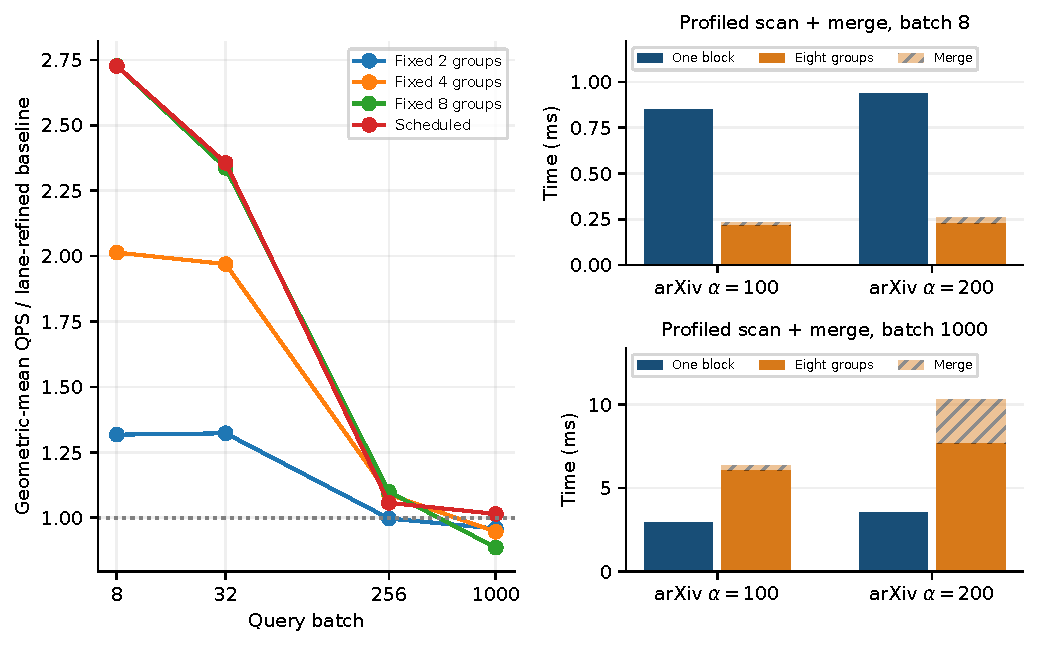
\includegraphics[width=\linewidth]{ch7/batch_execution.pdf}
\caption[Batch-dependent execution regimes]{Execution regimes. Left: fixed shared-bound group counts and
scheduled execution relative to the lane-refined one-block baseline
(13 cells at small batches, 11 at batch 1,000). Right: paired scan and
merge profiles at batches 8 and 1,000 for arXiv budgets 100 and 200.
Hatching denotes merge time. The right panels use the independent-bound
scan experiment; they explain a cost, not the scheduler's entire speedup.}
\label{fig:7-batch}
\end{figure}

\subsection{A fixed rule evaluated on further configurations}

The scheduler follows the fill/skew rule and pseudoquery calibration
in \cref{sec:5-5}. Four configurations set the constants before the
additional configurations were measured.


\begin{table}[tbp]
\centering
\caption[Integrated execution and scheduling gains]{Integrated execution gains over v61 L16. Entries are geometric
 means of per-cell median paired speedups from five rounds. ``Held out''
 excludes the four configurations used to set the rule; it means held-out
 configurations, not the budget experiment's held-out query split.}
\label{tab:7-scheduling}
\small\setlength{\tabcolsep}{4pt}
% Generated by scripts/build_ch7.py; do not edit numbers manually.
\begin{tabular}{@{}rrrrrrr@{}}
\toprule
Batch & Cells & $g_s=2$ & $g_s=4$ & $g_s=8$ & Scheduled & Held out \\
\midrule
8 & 13 & 1.318 & 2.014 & 2.728 & 2.727 & 2.930 \\
32 & 13 & 1.323 & 1.970 & 2.337 & 2.356 & 2.560 \\
256 & 13 & 0.997 & 1.090 & 1.099 & 1.057 & 1.041 \\
1000 & 11 & 0.959 & 0.947 & 0.886 & 1.015 & 1.012 \\
\bottomrule
\end{tabular}

\end{table}

\Cref{tab:7-scheduling} gives the paired gains and evaluation subsets.
The small-batch means use thirteen configurations; batch 1,000 uses
eleven because Stella has 999 queries, with nine/seven held-out
configurations respectively. Scheduling retains the batch-8 benefit
while protecting full-batch execution: fixed eight groups fall to
$0.886\times$ at batch 1,000. The largest scheduler regret is
1.217 on BGE at batch 256, showing that candidate-count CV omits
some traversal and selection costs.

Vogue illustrates both the value and limits of the skew feature. Its E1
candidate-count CV ranges from 0.338 to 0.622 as probes change, forcing
four groups at batch 1,000. The integrated path/one-block ratio ranges
from 0.895 to 1.175. It loses at $(n_{\rm probe},\alpha)=(16,16)$,
$(16,64)$ and $(32,64)$, with ratios 0.955, 0.895 and 0.955.
Candidate-count dispersion alone does not encode absolute per-query work;
the rule can add overhead to these low-probe cases while enabling Vogue's
0.97 cross-system lead in \cref{sec:7-2}. Both failures expose
decomposition costs missing from the CV feature.

Finally, correctness is checked independently of timing. Across 250
variant/configuration comparisons and 234,320 query comparisons, the
integrated campaign reports no non-tie primary-selection differences and
no different final identifier sets. Final order can differ at ties;
the entire campaign should not be described as universally bit-identical.
The throughput results concern sequential, synchronous submissions and
do not establish tail latency under an open-loop arrival process.

\section{Cold Construction, Resident Memory and Tested Scale}
\label{sec:7-7}

RQ1 is assessed through cold construction, resident memory and completed
large-dataset searches; the E1 memory comparison also informs RQ4.

\subsection{Cold builds and the lifecycle boundary}

Unlike the cached search sweeps, \cref{tab:7-build-memory} uses three
normal empty-cache train/add repetitions per dataset.
Vogue's training is 298--303\,ms, so its normal total is about 0.56\,s;
the archived 1.33\,s total (including 1.056\,s training) is an unusually slow single observation.
Stella's normal totals are 10.54--10.65\,s, close to the historical
10.40\,s record.

\begin{table}[tbp]
\centering
\caption[Cold construction and resident memory]{Cold JHQ construction and separately measured resident memory.
Train/add are component medians of three supplementary normal builds;
Total is the median paired sum. Memory comes
from v71's two-group, 128-probe, $\alpha=100$ runs and includes context
and workspace. ``Residual'' is the modelled residual-code share of the
measured used total, not the fraction read per query.}
\label{tab:7-build-memory}
\small\setlength{\tabcolsep}{3pt}
% Generated by scripts/build_ch7.py; do not edit numbers manually.
\begin{tabular}{@{}lrrrrrr@{}}
\toprule
Dataset & Train s & Add s & Total s & Used GiB & Raw GiB & Residual \\
\midrule
Vogue & 1.06 & 0.27 & 1.33 & 1.47 & 2.67 & 45.4\% \\
arXiv & 0.59 & 0.52 & 1.10 & 2.58 & 6.45 & 62.5\% \\
OpenAI-1536 & 0.64 & 0.38 & 1.01 & 2.39 & 5.72 & 59.7\% \\
OpenAI-3072 & 1.34 & 0.65 & 1.99 & 4.14 & 11.43 & 69.0\% \\
BGE & 3.75 & 3.67 & 7.42 & 11.93 & 38.50 & 80.7\% \\
Stella & 3.74 & 6.67 & 10.40 & 20.44 & 67.81 & 82.9\% \\
\bottomrule
\end{tabular}

\end{table}

Construction and startup boundaries follow \cref{sec:3-3,sec:a-e1-protocol};
\cref{fig:7-build} compares these repetitions with baseline configurations.


\begin{figure}[tbp]
\centering
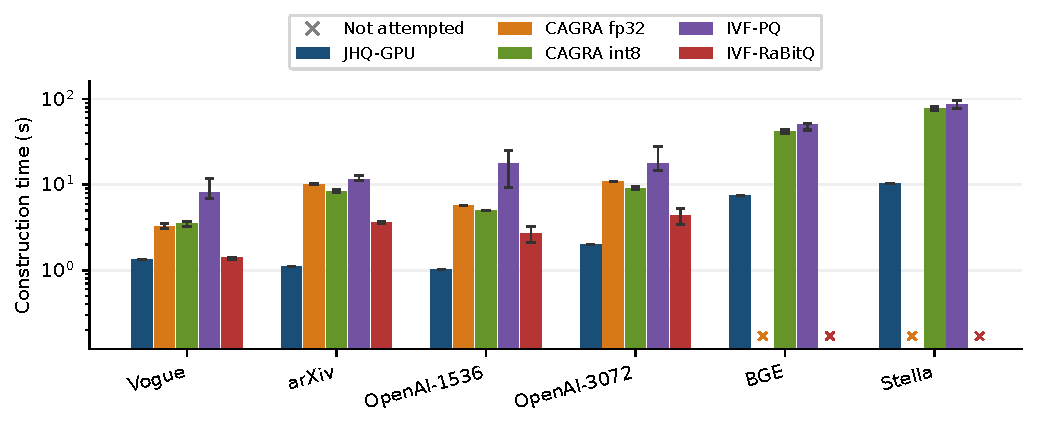
\includegraphics[width=\linewidth]{ch7/construction.pdf}
\caption[Recorded construction costs]{Recorded construction costs, with CAGRA int8 included. JHQ is
the median and range of three supplementary normal cold builds with warm
input pages; other bars are medians across successful
measured index configurations, with minimum--maximum whiskers. Int8
includes dataset quantization; RaBitQ excludes the required serialization
round trip. Missing large-dataset bars denote unattempted configurations,
not measured build failures. The vertical axis is logarithmic.}
\label{fig:7-build}
\end{figure}

On Stella, successful isolated CAGRA int8 builds take approximately
74.55 and 82.45\,s including dataset quantization, depending on graph
degree; the measured IVF-PQ build median is 86.59\,s across its three
configurations. JHQ's 10.54--10.65\,s repeated interval is substantially shorter under the
reported boundaries. Downstream quality and resident cost are evaluated
separately.


Five independent builds give a maximum fixed-point recall range
of 0.0012 on arXiv; normal timing uses three uninstrumented builds.
Startup is a broader boundary: Stella takes 18.2--18.6\,s with warm
input pages, versus 129.9\,s on the session-first read.
Twenty-millisecond device sampling observes 26.08\,GiB near BGE's
add entry and 22.58\,GiB during Stella's repack. BGE's three
assignment buffers total 12\,GiB in an earlier lifetime than the
23.05\,GiB gather payload (\cref{eq:4-assignment-scratch}); the two
allocations must not be summed as a simultaneous peak.

\subsection{Resident allocation and where compression helps}

\Cref{fig:7-memory} combines the component model in \cref{sec:4-4}
with measured resident totals. Its unattributed remainder is retained,
and the preceding construction measurements give the sampled peaks.


\begin{figure}[tbp]
\centering
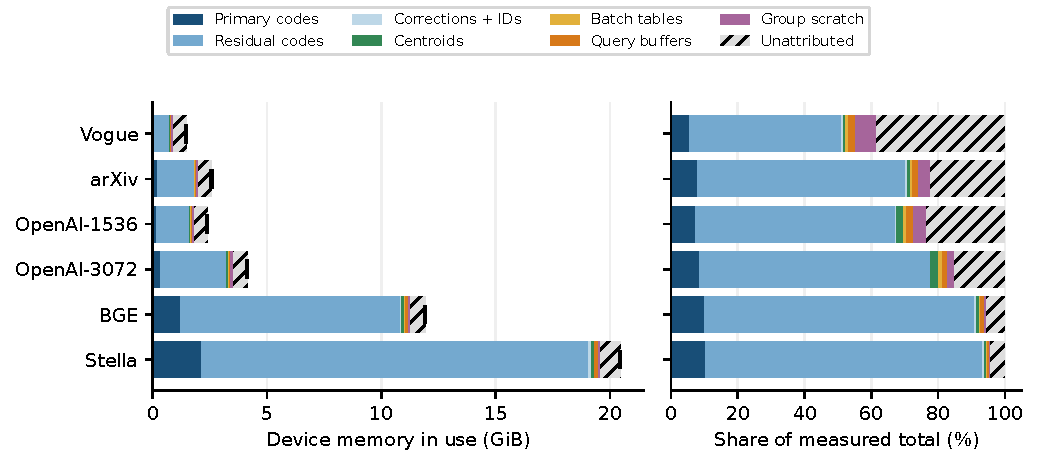
\includegraphics[width=\linewidth]{ch7/memory.pdf}
\caption[Resident-memory decomposition]{Resident-memory decomposition at two-group tables, 128 probes
and $\alpha=100$. Component sizes are modelled, markers are measured used
totals, and hatching is the unattributed remainder. The totals include
context and workspace. The preceding construction measurements give sampled peaks; these
resident markers are not peaks.}
\label{fig:7-memory}
\end{figure}

Residual codes account for 80.7\% of BGE's 11.93\,GiB and 82.9\%
of Stella's 20.44\,GiB measured totals. Raw FP32 vectors alone would
require 38.50 and 67.81\,GiB. These resident totals include context
and query workspace; lowering $\alpha$ changes residual access rather
than the stored array. The component model is in \cref{sec:4-4}.

The reserved group workspace is about 93.8\,MiB even on the one-block
path, for batch capacity 1,024 and up to eight groups. Actual group
count therefore does not determine allocated capacity. Construction
peaks and after-build index deltas also exclude different allocations;
some baseline search pools are initialised after index-memory measurement.

The E1 measurements provide a separate cross-system view in
\cref{tab:7-e1-memory}. Subtracting the baseline-measured 507.2\,MiB
context from JHQ's process total gives approximately 0.29--0.39 of
CAGRA fp32's index allocation. JHQ's figure includes workspace, whereas
CAGRA's is the build-time index delta. These are parameter-sweep ranges,
not memory-matched recall points or a comparison of equal peak budgets.
The CAGRA int8 allocations in the same table are of a similar order to
JHQ's: compression relative to fp32 is shared by competing designs.
The component model in \cref{tab:4-bytes} explains this comparison.

\begin{table}[tbp]
\centering
\caption[E1 allocation ranges]{E1 allocation ranges. JHQ is process total minus a 507.2\,MiB
context estimate, including query workspace; both CAGRA columns are index
allocations measured during build. Ranges cover the parameter sweep.}
\label{tab:7-e1-memory}
\footnotesize\setlength{\tabcolsep}{4pt}
% Generated by scripts/build_ch7.py; do not edit numbers manually.
\begin{tabular}{@{}lrrr@{}}
\toprule
Dataset & JHQ net process GiB & CAGRA fp32 index GiB & Ratio range \\
\midrule
Vogue & 0.90--1.01 & 2.89--2.91 & 0.31--0.35 \\
arXiv & 2.01--2.19 & 6.84--6.98 & 0.29--0.32 \\
OpenAI-1536 & 1.79--2.33 & 5.95--5.97 & 0.30--0.39 \\
OpenAI-3072 & 3.54--3.82 & 11.67--11.68 & 0.30--0.33 \\
\bottomrule
\end{tabular}

\end{table}

\subsection{Large-dataset feasibility and competitive regions}

BGE contains 10,091,524 vectors and Stella 17,776,615, both with
1,024 dimensions and 32,768 IVF lists. Stella's queries are sampled from
the corpus; its result therefore characterizes that benchmark rather
than an independently collected external-query distribution.
\Cref{fig:7-large} includes
successful CAGRA int8 and IVF-PQ measurements. Full-precision CAGRA,
RaBitQ configurations and FP32 brute force were not attempted in the
large-scale comparison when their computed storage requirements exceeded
the available device capacity. Those omissions are planned feasibility
exclusions, not observed out-of-memory errors or measured recall failures.

\begin{figure}[tbp]
\centering
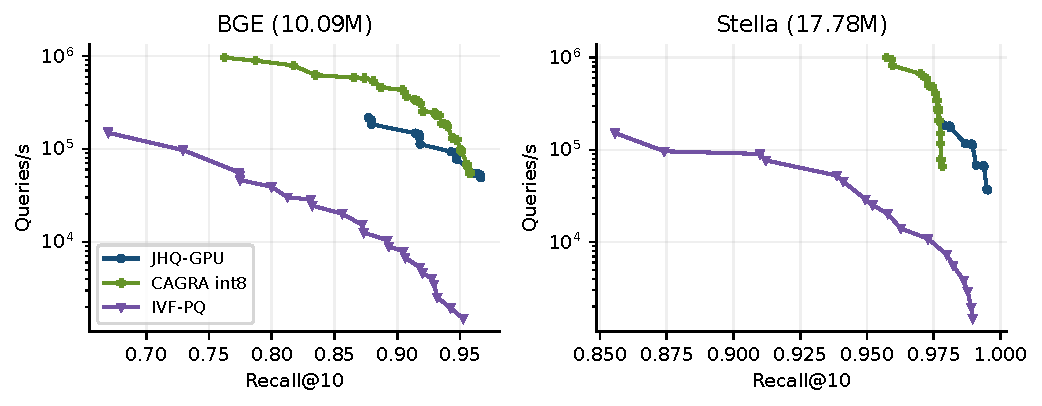
\includegraphics[width=\linewidth]{ch7/large_frontiers.pdf}
\caption[Large-dataset search frontiers]{Large-dataset host-to-host frontiers, including the successful
isolated CAGRA int8 reruns. BGE uses 1,000 queries and Stella 999. An
endpoint is the end of the tested grid, not an intrinsic recall limit.}
\label{fig:7-large}
\end{figure}

Successful isolated reruns show that CAGRA int8 fits Stella in the
tested configurations. On BGE, int8 is approximately $1.35$--$2.96\times$
faster at the sampled common targets 0.88/0.90/0.92/0.94/0.95. At its
measured maximum recall 0.9579, JHQ's interpolated QPS is $1.086\times$
int8's. Thus the advantage changes direction near the high-recall end.
The maximum tested recalls are 0.9579/0.9783 for int8, 0.9663/0.9952
for JHQ and 0.9525/0.9896 for PQ on BGE/Stella.

On Stella, one concrete high-end comparison is 185.4 kQPS at recall
0.978679 for JHQ versus 66.3 kQPS at 0.978278 for int8, a $2.80\times$
rate ratio with slightly different recall. This is an explicit pair of
measured points, not a uniform matched-recall gain: much of JHQ's
higher-recall region has no int8 coverage, and JHQ's highest-recall
points trade throughput for quality. Corrected-run exclusions and
harness diagnostics are recorded in Appendix~\ref{app:reproducibility}.

The experiments demonstrate single-GPU search over 17.78 million vectors
and useful high-recall operating regions. Multi-GPU execution and
scaling at a fixed data distribution remain untested. Construction
memory samples leave shorter allocation transients unresolved near
device capacity. Stella uses its actual 999-query pool.

\section{Numerical Robustness, Anomalies and Recall Attribution}
\label{sec:7-8}

The robustness checks qualify the RQ2 exactness claims, the RQ3 risk
assessment and the small cross-system margins in RQ4.

\subsection{Quality resolution and repeated execution}

With $k=10$ and 1,000 queries, one recovered neighbour changes aggregate
Recall@10 by $10^{-4}$; with 500 held-out queries the resolution is
$2\times10^{-4}$. Stella's 499-query split has a slightly coarser
resolution. This discretization is not an uncertainty interval, but it
helps interpret the small differences reported above. A fourth-decimal
change may represent only one or two result slots, while a small mean
loss can still hide several queries with substantially changed answers.

Repeated calls and repeated index builds answer different questions.
E1 retains 369 baseline repeat-call identifier flags, including tie-order
changes; these points remain in the frontiers. The 401-count convention
and cross-protocol checks are separated in \cref{sec:a-e1-protocol}.

Five-round ranges describe timing within a fixed build. A separate
frontier-slope calculation quantifies sensitivity to a horizontal recall
shift: continuous log-QPS segments adjacent to 0.97 imply about
1.01--3.17\% rate change per $10^{-3}$ recall, before applying the
near-target snapping convention. The supplementary five-build recall ranges are 0.0008 for Vogue,
0.0012 for arXiv, 0.0004 for OpenAI-1536 and 0.0002 for OpenAI-3072
at fixed operating points. Applied purely as horizontal sensitivity
scales to the local slopes, these imply changes of order a few percent,
rather than the larger OpenAI fp32-CAGRA margin. The experiment does
not repeat whole frontiers or baseline builds; it therefore supports
local stability assessment, not a universal bound on matched ratios.
The precision intervention in \cref{sec:7-precision} directly establishes
that the OpenAI advantage survives removal of TF32 under its stated
cached-model boundary. ArXiv and the LUT near ties retain their narrower
interpretation.

Across each dataset's RaBitQ configurations, the median five-round
range divided by median QPS is 3.79\%, 3.34\%, 2.87\% and 5.25\%
for Vogue, arXiv, OpenAI-1536 and OpenAI-3072. These descriptive spreads
are comparable in scale to the small Vogue advantage, rather than
confidence intervals for its matched ratio. Raw call traces also contain
long calls, including occasional 30--60\,ms observations in otherwise
faster configurations. As a sensitivity check, recomputing QPS as
$10^6/\operatorname{median}(\text{call latency in ms})$ for a
1,000-query call reduces the influence of long calls.
At recall 0.97, the resulting JHQ/RaBitQ ratios are 1.063, 0.995,
1.118 and 1.100. The three favourable directions and arXiv near parity
remain, so the result is not solely a consequence of long calls.

\subsection{Exactness is attached to a particular stage}
\label{sec:7-recall-attribution}

The stage contracts in \cref{tab:5-query-stages} distinguish computed-score
selection from raw-space kNN; lane rounding, cutoff ties and process
variation qualify different stages.


The archived reconstruction pilot measures the remaining gap to
full-probe reconstructed scoring.
Across seven workload--budget arms of 128 queries each, scoring all
probed candidates in FP64 improves recall over GPU outputs at selected budgets by
0--0.002344. For arXiv at 128 probes, $\alpha=200$ matches the full-IVF
reconstructed answer set on all 128 queries. At 100, the recall is
0.9734375 versus 0.9750 for full-IVF scoring: an additional 0.0015625
budget deficit beside the joint routing/reconstruction deficit of
0.0250 (\cref{sec:6-2}). These are pilot-specific aggregate differences;
the seven arms include two budgets on one dataset--probe workload.
FP64 reconstructed scoring also differs from the GPU arithmetic, so the
pilot does not isolate a pure budget effect in every arm. Separating
routing from representation requires additional stage-wise GT coverage.

% Section structure adapted from 6.pdf; draft prompts are not thesis prose.
\chapter{Discussion, Limitations and Future Research}
\label{ch:discussion}
\draftnote{Synthesize supported findings, analyse two relevant negative designs, and state internal and external validity limits.}

\section{Three Cross-Layer Insights}
\label{sec:8-1}
\draftnote{Develop the supported links between representation and execution, parallelism and repeated work, and execution cost and the value of budget reduction.}

\section{Two Deep Negative-Result Case Studies}
\label{sec:8-2}
\draftnote{For two case studies, state hypothesis, alternatives, test conditions, observations, and stopping decision. Label isolated GPU, offline, estimated, and untested evidence.}

\section{Threats to Internal and External Validity}
\label{sec:8-3}
\draftnote{Write this section using the verified methods and evidence. State the relevant conditions and connect the argument to its research question.}

\section{Original Testable Research Directions}
\label{sec:8-4}
\draftnote{Write this section using the verified methods and evidence. State the relevant conditions and connect the argument to its research question.}

\section{Conditional Deployment Recommendation}
\label{sec:8-5}
\draftnote{Write this section using the verified methods and evidence. State the relevant conditions and connect the argument to its research question.}

% Section structure adapted from 6.pdf; draft prompts are not thesis prose.
\chapter{Conclusion}
\label{ch:conclusion}
\draftnote{Answer the research questions using only results already established. Do not introduce new measurements or contributions.}

\section{Answers to the Four Research Questions}
\label{sec:9-1}
\draftnote{Write this section using the verified methods and evidence. State the relevant conditions and connect the argument to its research question.}

\section{Closing Principle and Outlook}
\label{sec:9-2}
\draftnote{Write this section using the verified methods and evidence. State the relevant conditions and connect the argument to its research question.}


\clearpage
\phantomsection
\addcontentsline{toc}{chapter}{Bibliography}
\bibliographystyle{plainnat}
\bibliography{references}

\appendix
\chapter{Reproducibility and Experiment Manifest}
\label{app:reproducibility}
\section{Source and Build Environment}
\draftnote{Record immutable source commits, compiler options, GPU and host
details, dependencies, and how the binaries were built. Distinguish the thesis
repository from the implementation repository.}
\section{Data and Trained States}
\draftnote{Document dataset identifiers, preprocessing, query and GT hashes,
split rules, trained-state cache identities, and exclusions.}
\section{Result-to-Figure Mapping}
\draftnote{Map every empirical figure to its raw files, analysis script,
configuration, metric definition, and reproduction command. Explain exactly
what cold construction includes.}

\chapter{Supplementary Results and Correctness Checks}
\label{app:supplementary}
\section{Complete Parameter Grids}
\draftnote{List method-specific tuning grids, invalid or unavailable settings,
and reasons for unattempted configurations.}
\section{Correctness and Numerical Checks}
\draftnote{Include reference comparisons for encoding, LUT factorisation,
primary selection, probe selection, and refinement. Separate numerical,
algorithmic, and memory-safety evidence.}
\section{Additional Results and Negative Designs}
\draftnote{Include secondary results with evidence status: integrated system,
isolated GPU measurement, offline replay, analytical estimate, or untested idea.}

\chapter{Contributions and Tool-Use Record}
\label{app:author-tools}
\draftnote{Use the form of disclosure required by Canvas. The tables below
are a record template, not an attestation that any particular verification
was performed. Replace all entries with a truthful account.}
\section{Contribution Record}
\begin{longtable}{@{}p{0.22\textwidth}p{0.34\textwidth}p{0.34\textwidth}@{}}
\toprule
Work component & Contributor and role & Supporting record \\
\midrule
\endhead
\textit{To complete} & \textit{To complete} & \textit{To complete} \\
\bottomrule
\end{longtable}
\section{Generative-AI Assistance}
\begin{longtable}{@{}p{0.19\textwidth}p{0.34\textwidth}p{0.37\textwidth}@{}}
\toprule
Tool and date & Purpose and scope & Prompt record and human review \\
\midrule
\endhead
\textit{To complete} & \textit{To complete} & \textit{To complete} \\
\bottomrule
\end{longtable}

\ifdraftthesis
  % Included only while \draftthesistrue. It is not thesis content.
\chapter{Template Examples --- Draft Only}
\label{app:template-examples}
This appendix demonstrates the available formatting. It is omitted when
\verb|\draftthesisfalse| is selected in \texttt{config/metadata.tex}.

\section{Citations and Cross-References}
Use \verb|\citet{jhq}| for a narrative citation: \citet{jhq}.
Use \verb|\citep{pq,cagra}| for a parenthetical citation \citep{pq,cagra}.
Examples: \cref{fig:example-pipeline,tab:example-manifest,eq:example-disagreement}.
The bibliography entries are copied from the existing ADC source; review their
metadata before submission.

\section{A Source-Native Diagram}
\begin{figure}[tbp]
\centering
\begin{tikzpicture}[
  node distance=5mm,
  stage/.style={draw=ThesisNavy,rounded corners=2pt,fill=ThesisNavy!4,
    minimum height=10mm,text width=26mm,align=center,font=\small},
  link/.style={-{Latex},draw=ThesisNavy}]
  \node[stage] (route) {IVF routing};
  \node[stage,right=of route] (screen) {Primary screening};
  \node[stage,right=of screen] (refine) {Residual refinement};
  \node[stage,right=of refine] (output) {Final top-$k$};
  \draw[link] (route) -- (screen);
  \draw[link] (screen) -- (refine);
  \draw[link] (refine) -- (output);
\end{tikzpicture}
\caption{Formatting example: a schematic query path. Replace or extend it
with the verified execution boundaries of the implementation.}
\label{fig:example-pipeline}
\end{figure}

% A real PDF figure can be inserted without copying any local absolute paths:
% \begin{figure}[tbp]
%   \centering
%   \includegraphics[width=\linewidth]{frontier.pdf}
%   \caption{State version, dataset, hardware, k, batch, timing boundary,
%     varied parameters, uncertainty, and interpolation when relevant.}
%   \label{fig:frontier}
% \end{figure}

\section{Tables}
\begin{table}[tbp]
\centering
\caption{Example manifest fields. This table contains no experimental results.}
\label{tab:example-manifest}
\begin{tabularx}{\linewidth}{@{}lX@{}}
\toprule
Field & What to record \\
\midrule
Source & Immutable commit and build configuration \\
Index & Trained-state identity and input hashes \\
Timing & Host-to-host or device-resident boundary \\
Quality & Metric, ground truth, and held-out split \\
Evidence & Raw log and analysis-script path \\
\bottomrule
\end{tabularx}
\end{table}

\section{Equations and Proofs}
\begin{equation}
 D(\alpha)=\sum_{q\in Q_s}
  \left[k-\left|R_\alpha(q)\cap R_{\max}(q)\right|\right].
 \label{eq:example-disagreement}
\end{equation}
The environments \texttt{definition}, \texttt{lemma}, \texttt{proposition},
and \texttt{proof} are available. For example:
\begin{definition}[Strict total ranking key]
A ranking key specifies how to order unequal scores and how to break ties.
\end{definition}
% \begin{proposition}[Descriptive title]
%   State the precise premises and claim here.
% \end{proposition}
% \begin{proof}
%   Give the argument, including floating-point and tie assumptions.
% \end{proof}

\section{Pseudocode and Code}
The table below gives a package-light pseudocode layout; replace its contents
with the actual method and keep correctness premises in the surrounding text.
\begin{table}[tbp]
\centering
\caption{Pseudocode layout example.}
\begin{tabularx}{\linewidth}{@{}rX@{}}
\toprule
Line & Operation \\
\midrule
1 & Read the input and validate the stated preconditions. \\
2 & Compute the intermediate result. \\
3 & Return the output and specify its semantics. \\
\bottomrule
\end{tabularx}
\end{table}
\begin{lstlisting}[language=C++,caption={Code-listing format example.}]
// Use only short excerpts that help explain a design.
// Keep full implementations in the reproducibility artifact.
void search();
\end{lstlisting}

\fi
\end{document}
